% vim: syntax=tex

%\paragraph{}

%\begin{prose}


%\cleardoublepage
\section*{}
\markboth{}{Liminaire}
\thispagestyle{empty}
%\sectionmark{Genèse}
\addcontentsline{toc}{section}{Liminaire}
{\em\small
\parshape=7
0pt \textwidth
0.19\textwidth 0.81\textwidth
0.21\textwidth 0.79\textwidth
0.22\textwidth 0.78\textwidth
0.22\textwidth 0.78\textwidth
0.05\textwidth 0.95\textwidth
0pt                \textwidth
%\noindent\raisebox{-\height}[0pt][0pt]{
\includepdf[pages={1}]{lettrine-A-diborgo.pdf}}%
%\noindent\raisebox{-\height}[0pt][0pt]{truc}%
\noindent{}\raisebox{-\height+0.565cm}[0cm][0pt]{
\hspace{-1.7cm}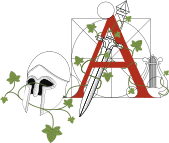
\includegraphics[width=0.36\textwidth]{lettrine-A-diborgo-grand.pdf}}\addcontentsline{lof}{figure}{Lettrine \autonym{A} aux divines proportions d’après l’alphabet de di~Borgo accompagné de lierre, lyre, casque corinthien, et dague}%
\hspace{-0.2cm}{\color{rouge}\em\textsc{l’origine de ce diwan,}} oh oui, il y’avait certes toute l’inspiration qui est y est à l’œuvre, de ces petits riens du quotidien que l’on ne sait précieux que lorsqu’on les perds. Instants fugaces si bien observés par Bashō qui n’ont d’autre défauts que de nous en laisser insatiables comme l’a relevé Lissān~al-Ḋḋīn, et ce parcequ’ils sont insaisissables. Or c’est malgré tout \incise{non pas en vain, espéré-je} qu’à travers la poésie je comptais en capter quelque instantané comme l’aurait fait \fallbackserif{Ȝ}omār Xayām ou sans doute même… Louis \textsc{Daguerre}.

%\lettrine[lines=5,image=true, lraise=0, findent=0em, loversize=0.25]{lettrine-A-diborgo.pdf}{\color{rouge}l’origine de ce diwan,} oh oui, il y’avait certes toute l’inspiration qui est y est à l’œuvre, de ces petits riens du quotidiens que l’on ne sait précieux que lorsqu’on les perds. Instants fugaces si bien observés par Bashō qui n’ont d’autre défauts que d’être insaisissables comme l’a relevé Lissān~al-Ḋḋīn, et c’est malgré tout en vain qu’à travers la poésie je comptais en capter un instantané comme l’aurait fait \fallbackserif{Ȝ}omār Xayām ou sans doute même… \textsc{Daguerre}.

	Or, ces infimes détails, présents de l’Éternel, s’ils sonnent comme un \xenism{carpe diem} c’est  que leur valeur ne s’acquière que parcequ’éphémères, et ils ne peuvent alors véritablement se jauger qu’à la faveur des deux principales activités de l’homme depuis la nuit des temps consacrant sa finitude au sein de sa grandeur que sont l’amour et la guerre. Pulsion de vie, pulsion de mort. Deux faces d’une même pièce, chacune variante de l’autre. Le titre de cet ouvrage aurait sans doute gagné à être donné en langue arabe où ces deux concepts se disent \xenism{ĥobb} \textarabic{حبّ} et \xenism{ĥarb} \textarabic{حرب} qui, fort prodigieusement ne varient que d’une seule lettre, révélant une assonance éloquente. Rappellerais-je à cet égard la parenté étymologique entre \xenism{bellum} (\enquote{guerre}) et \xenism{bellus} (\enquote{beau}) ⸮

	Il est même étrange que nombre de civilisations aient écarté les femmes de la guerre \incise{sauf, hélas, en tant que victimes}, alors qu’authentiquement elles auraient fait d’excellentes stratèges autant que de féroces combattantes. Pourtant, l’intuition des Grecs fit bien Aphrodite et Ares non seulement frère et sœur ainsi qu’amants mais encore frères de sang lorsqu’au chants \textsc{v} et \textsc{vi} de l’\work{Iliade} la flèche du téméraire Diomède les blessa tous deux mêlant ainsi leur sang.

L’amour est assurément une lutte, tandis que la guerre procède par la séduction. Sun Tzu ne dit-il pas si bien \enquote{Faîtes en sorte que vos prisonniers se retrouvent mieux chez vous qu’ils ne le seraient dans leur propre camp}, leçon dont s’instruirait tout aussi bien un amant ? La rime y répond.

Il y’avait tout cela, dis-je, au fondement de mes quelques vers. Mais en réalités, il n’aurait jamais été pris la peine de saisir le qalām, le stylographe, le porte-plume, la bombe de peinture aérosol, ou le clavier, s’il n’y avait pour transcender le tout, ma plus énamourée maitresse, celle qui me teint éveillé tant de nuits et pour qui le premier poème ne pouvait qu’être dédié.
}
%\end{prose}

%\versehangrightsquare
\poemtitle{Complainte de l’insomniaque}
\begin{verse}
À mes nuits, elle est la plus fidèle amante\\
Puisqu’à nos noces les témoins se sont assoupis.\\
Et si souvent, de ses charmes elle me tente,\\
C’est qu’elle se faufile et se love jusqu’à mon lit.

Jalouse, elle évince une à une ses rivales,\\
Verveine, camomille, tisane, aucune ne l’accable.\\
Mais toi, café son acolyte, lui ouvre les volets\\
À chaque fois qu’elle trouve porte fermée.
\end{verse}

%\paragraph{}
\begin{prose}
Car enfin, ne vous étonnez pas qu’au toucher, ce livre vous paraisse quelque peu humide, c’est qu’il est tout le long traversé par une intarissable nappe de café.
\end{prose}

%\paragraph{}
\begin{prose}
D’ailleurs, c’est devant la porte d’un établissement-café où j’attendais quelqu’un que m’apparut le haïku suivant. Au dessus d’un recueil de Bashō que je lisais, se trouvait une bouche d’égout.
\end{prose}

\poemtitle{De la bouche d’égout}
\begin{verse}
La bouche d’égout,\\
Les jambes de l’élégante\\
Y ont rendez-vous.
\end{verse}

\poemtitle{De la nappe de café}
\begin{verse}
Sur sillon dorsal,\\
Fuie la nappe de café\\
Des cheveux châtain.
\end{verse}

\poemtitle{Du cheveux sur la manche}
\begin{verse}
Café à la main,\\
Sur la manche de ma veste,\\
Un cheveux châtain.
\end{verse}

%\paragraph{}
\begin{prose}
C’est plus tard dans la soirée que les vers de Lissān~al\,Ḋḋīn ibn~al\,Xatīb, m’inspirèrent. Ils étaient si à propos qu’ils me semblaient que de son \textsc{xiv}\ieme{} siècle il me les destinait.
\end{prose}

\poemtitle{Flamme dans la nuit}
\begin{verse}
Ô nuit, drape de sombreur nos délits\\
Qui sous le voile noir cueillent un fruit.\\
Ô yeux\endnote{Dans la poésie et la musique arabe, les mots apostrophés \autonym{ô nuit} (\textarabic{يا ليل}) et \autonym{ô yeux} (\textarabic{يا عين}), sont d’ordinaire utilisés comme vocalises.}\label{foot.vocaliseYeuxNuit}, ne soyez  éblouis du feux\\
Qui, ardent, trahi les amants pieux.
\end{verse}

\poemtitle{Mélancolie}
\begin{verse}
Les larmes que tu extirpa de mon âme\\
Ne suffirent pas à calmer le brasier.\\
Et je noierais mon chagrin dans le café\\
S’il n’avait apprit à y nager, l’infâme.
\end{verse}

\poemtitle{Parole}
\begin{verse}
Un seul mot sucré d’elle\\
Vaut mieux que mille paroles.\\
Il emprunte aux alvéoles\\
La gelée et le miel.
\end{verse}

\poemtitle{Âme de cristal}
\begin{verse}
Ce sont des pleures fatales qu’elle pousse,\\
À chaque arpège d’Astor Piazzolla.\\
Mais, sur ses joues, les perles qui s’éclaboussent,\\
Indélébiles, sont des larmes de verre\\
Qui pleuvent pareilles au pianola\\
Aussi irrépressibles et régulières.

L’on ne peut les essuyer ni les briser\\
Mais leur point faible en est le filament\endnote{Allusion aux larmes de verre, artefact verrier dont le bulbe résiste à des chocs puissants tandis que le filament, s’il est rompu fait éclater l’ensemble.}\\
Qui, rompu, rend les plaies cicatrisées\\
Et les larmes étoiles du firmament.

Mais que peuvent verser d’autre, ses yeux ivrognes\\
Elle qui est une bouteille de Bologne\endnote{Ses bouteilles ont la particularité de résister à des coups de masse exercés depuis l’extérieur alors que le moindre objet en contact avec l’intérieur pulvérise toute la bouteille.}\\
Solide et imprenable de l’extérieur\\
Mais pourtant vulnérable de l’intérieur ?
\end{verse}

\poemtitle{Du cheveux d’airain}
\begin{verse}
Des cheveux d’airain\\
Tombant sur les reins,\\
Et je prend congé du monde.
\end{verse}


\poemtitle{Le sentier pavé d’or}
\begin{verse}
Tous les rayons du soleil se recueillent\\
Là où s’illumine un sur corridor\\
Jalonné d’accrocs, d’embûche et d’écueils.\\
Et c’est vêtu de haillons et pieds nus\\
Que s’emprunte le sentier pavé d’or\\
Le sentier glorieux qui mène aux nues.
\end{verse}

\poemtitle{Jardins d’Al-Andalous}
\begin{verse}
Célébrée dans les vers de Lissān~al-Ḋḋīn\endnote{Lissān~al-Ḋḋīn écrivit le muwachaĥ \work{Jadaka al-ṙaytu} faisant montre de nostalgie envers sa vie à Al-Andalous.}\\
Et portée par la voix de Juan Martin\endnote{Juan Martin interpréta le muwachaĥ andalous du \work{Lammā Bāda} dans son album \work{Musica Alhambra} parrut en 1998.},\\
Seuls l’oud et le kanoun\endnote{De l’arabe \textarabic{قاﻧﻮﻥ}. Instrument à cordes pincées, de la famille des cithares sur table.}\label{foot.kanoun} nous font parvenir\\
L’apaisant clapotement de tes fontaines.\\
Al-Andalous, si proche mais si lointaine,\\
Je souris encore à ton seul souvenir.

Qui des Almoravides aux Almohades,\\
Demeura fort belle jusqu’aux taïfas\\
Et l’est toujours malgré la Reconquista\\
Même si elle te porta l’estocade.

Car la prise de  Moussa Ibn Noçaïr\endnote{Wali et général du calife omeyade. Personnalité de premier plan dans la conquête d’Al-Andalous.}\\
Est, à la poésie et l’architecture,\\
Non le berceau mais plus encore l’ovaire\\
D’où bourgeonneront bientôt mille cultures.

Et l’étoile depuis trop longtemps éteinte\\
Qui est encore visible dans le ciel\\
Est semblable à tes beautés inertielles,\\
Celles dont nous parvient encore l’emprunte.

Plus que jamais prévaut le dit d’Alarcos\endnote{La devise de l’émirat de Grenade qui fut par la suite reprise par les différentes entités politiques d’Al-Andalous jusque sur leurs armoiries qui est \xenism{Wa la ṙāliba illa Allah.} (\enquote{Et il n’y a de vainqueur qu’Allah}) était frappée sur les bannières des armées musulmanes lors de la bataille d’Alarcos. D’ailleurs, les armoiries nasrides eurent ceci de singulier que, malgré les contacts intenses entre Arabo-musulmans et Européens, que ce soit à travers les croisades, la présence musulmane en Italie et en Sicile, ou l’invasion des territoires byzantins, aucune entité Arabo-musulmane ne jugea utile d’adopter la pratique occidentale de l’héraldique avant le XX\ieme{} siècle, à l’exception notable justement de l’émirat de Grenade. Lequel d’ailleurs ne fit qu’y faire figurer inlassablement son implacable devise.},\\
Funeste oracle digne de la Pythie\endnote{Pythie de Delphe dont l’oracle équivoque à Crésus lui annonçait qu’après la bataille qu’il devait mener un grand empire allait s’effondrer. Après que Crésus ait mené sa bataille, un grand empire s’est effectivement effondré, le sien.}\\
Qui, gravé à l’envie sur les armoiries,\\
Rappelle ta disparition précoce\\
Car, partout jusqu’aux jardins de l’Alhambra,\\
Nous disons \xenism{Wa la ṙāliba illa Allah.}
\end{verse}

\poemtitle{Un baiser}
\begin{verse}
Ce n’était peut-être qu’un baiser\\
Mais il m’avait laissé bouche-bée.
\end{verse}

\poemtitle{Portes d’Al-Andalous}
\begin{verse}
Rapporte mes faits, Ibn Tumulus\endnote{Historien dont les chroniques sont le plus ancien témoignage sur la conquête d’Al-Andalous nous étant parvenu.}.\\
Elle me promeut en général\\
Et fait couler les nefs dans mon dos.\endnote{Allusion au général Tariq ibn~Zayad. Personnage d’importance centrale dans la conquête d’Al-Andalous au point qu’il donna son nom à Gibraltar (voulant dire montagne de Tariq). On raconte que suite à son débarquement en Hispanie, il craignit que ses soldats ne fuient devant le surnombre des Wisigoths et fit alors naufrager leurs bateaux en annonçant \enquote{La mer est derrière vous et l’ennemi devant vous.}.}

Rapporte sur de maints papyrus\\
Que me suffit d’elle un seul sépale\\
Pour prendre l’Espagne aux Wisigoth.

Rapporte et rappelle mordicus\\
Que lorsque son sourire s’étale\\
S’ouvrent les portes d’Al-Andalous.
\end{verse}

\begin{figure}[h]
\centering

\includegraphics[height=3cm]{armoiries-grenade.pdf}
\captionsetup{labelformat=empty}
\caption[Armoiries nasrides de Grenade, d’après un relief de l’Alhambra, dont l’écu se blasonne ainsi \xenism{De gueule à la bande d’or, sur laquelle est écrit en arabe cursif \enquote{\textarabic{لا غالب إلا الله}} (\xenism{Il n’y a de vainqueur qu’Allah}).}.]{}
\end{figure}

\poemtitle{Artisan de l’Alhambra}
\begin{verse}
Es-tu chirurgien esthétique ou graveur\\
Quand, du mur, ton bistouri ripa de sa lame\\
Et fut poinçon sur mon visage de rêveur,\\
Pour y écrire l’ivresse tel un qalām ?

Si les murs de l’Alhambra tu les fis fleurir,\\
Toi jardinier qui trace la calligraphie,\\
C’est sur mes traits que ta florale épigraphie\\
S’est prolongé quand j’ai esquissé un sourire.
\end{verse}

\poemtitle{De l’assise}
\begin{verse}
Quand elle s’assied\\
Que ses  reins se sont creusés,\\
Une poire est née.
\end{verse}

\poemtitle{La nymphe}
\begin{verse}
Même les hommes les plus intègres\\
Cèdent à sa silhouette allègre\\
Voulue par Dieu si belle, si belle\\
Que s’élèvent au ciel des arpèges,\\
Emportant loin les feuilles de liège,\\
Laissant en émoi la citadelle.
\end{verse}

\begin{prose}
Dans la nouvelle revue \enquote{Par ici la sortie}, Margaret \textsc{Artwood} nous parle d’une image iconique, sans doute même partagée par l’imaginaire de chacun, d’un chevalier qui \enquote{galope à bride abattue vers un château dont le pont-levis se relève \textelp{} cavalier et monture décrivent alors un saut prodigieux afin de franchir les douves}. Sans doute qu’à l’heure des changements suscités par la pandémie, cette scène mobilise des espoirs et probablement même une métaphore de l’instant opportun à saisir par l’humanité, celui où plus que jamais il convient de fixer du regard le pont-levis plutôt que de regarder en arrière.

Puisse alors de son \textsc{xi}\ieme{} siècle AÈC porter encore la voix de Pittacos de Mytilène qui disait déjà \enquote{Sache reconnaître le moment opportun} ; puisse-t-il se faire entendre de nous.

Compte à Margaret \textsc{Artwood} qui a voulu chercher cette scène que nous connaissons intimement tous, que nous avons certainement vu dans un film de chevalerie ou de cap et d’épée, nous apprend dans le \enquote{Time} que nous avons sans doute été victime d’un effet Mandella. Car elle n’a rien trouvé d’autre que des photos de voitures tombées dans un lac et un épisode de la panthère rose.
\end{prose}
\poemtitle{Kaïros — Le moment opportun}
\begin{verse}
Vous croyez que c’était un cavalier\\
Mais c’est un éclaire qui est passé.\\
Homme et monture à tout jamais liés,\\
Il vont au loin occire ou trépasser.

Voilà un bref instant non écrit de l’histoire,\\
De ces Point de bascule où le cours peut changer\\
Et emprunter une inattendue trajectoire.\\
Un moment que l’on ne peut saisir qu’enragé.

Un chevalier qui galope à bride abattue\\
Vers un château dont le pont-levis se relève,\\
\incise{Tant qu’il n’est pas encore clôt nul n’est battu}\\
Vers la muraille en approche, Il saisit son glaive.

Il n’y a qu’une infime chance, un interstice\\
Mais saisit, il parachèvera la victoire.\\
Tandis que les métrés restants sont un supplice,\\
Le pont qui s’élève encore peut toujours choir.

Il n’en est rien, car il est déjà hissé haut.\\
Cavalier et monture sautent prompts sur l’eau\\
D’un saut prodigieux et franchissent les douves,\\
Rayonnant dans les cieux de leur regard de louve.

Suspendus, leur élan est un instantané,\\
Car la physique qui hésite et se flagelle,\\
Entre la gravité et mouvement, chancelle\\
Et a tranché pour les deux en simultané.

Dans leur ascension et leur chute si frêles\\
Ils ne sont nul part ailleurs qu’accrochés au ciel\\
Ni dans le faussé, ni les sabot au planché.\\
Il sont à cet endroit là à jamais perchés.
\end{verse}

%\afterpage{\includepdf[pages={1},addtolist={1,figure,{Idéotexte de \autonym{Casablanca} (\textarabic{البيضاء})},ideocasa}]{casablanca-monochrome.pdf}}





\section*{Casablanca}
\markboth{}{Casablanca}
\addcontentsline{toc}{section}{Casablanca}


\begin{prose}
J’ai dû quitter tôt, trop tôt, mon agréable compagnie pour Casablanca où m’ont appelé certaines affaires. Ces affaires là n’étaient certes pas de la dernière urgence, mais comme j’ai toujours voulu caser quelque part cette phrase là qui donne l’impression d’être très occupé, eh bien j’ai trouvé que la situation y sied bien ! Toujours est-il que si la ville est certes réputée sale et polluée, par chance j’arrivai un jour où le ciel clair m’inspira le haïku :
\end{prose}

\poemtitle{Du ciel bleu}
\begin{verse}
D’entre les immeubles,\\
Jaillit une vérité,\\
Celle du ciel bleu.
\end{verse}

\begin{figure}[h]
\centering
\includegraphics[width=\textwidth]{casablanca-alone.pdf}
\captionsetup{labelformat=empty}
\caption[Idéotexte de \autonym{Casablanca} (\textarabic{البيضاء}.)]{}
\end{figure}

\poemtitle{Baiser ensoleillé}
\begin{verse}
Ayant sur l’horizon surfé,\\
Nos embrassades crépusculaires\\
Trempèrent  le soleil dans la mer\\
Tel un cookie dans le café\\
Si bien que des palmiers et néons\\
Ses lèvres m’ont laissé que néant.
\end{verse}

\poemtitle{Le déphasé}
\begin{verse}
Quelque part entre le néant et l’infini,\\
Enivré d’amour et d’insomnie,\\
Je me perdis en leur compagnie\\
Ne sachant dire s’il est midi ou minuit.

Chauve-souris dans une chambre anéchoïque\\
Que je suis, parmi les néons en mosaïque\\
Lorsque je somnambule de nuit dans la rue,\\
Perdu dans des endroits qui me sont bien connus.
\end{verse}

\poemtitle{À l’écoute}
\begin{verse}
À trop écouter mes désir\\
J’en suis devenu sourd\\
Et ma raison s’en vit gésir\\
Pourfendue par l’amour.
\end{verse}

\poemtitle{La ville catin}
\begin{verse}
Casablanca, aussi belle que tes catins\\
Qui, quoique distinctes, racolent en ton sein.\\
Dégoûtante comme celles des bas cartiers,\\
Princière comme les escortes de Gauthier\endnote{Cartier réputé bourgeois de Casablanca.}.
\end{verse}

\begin{prose}
Il y’a bien là force disgrâce et grande hideur mais elle est moins du fait des braves personnes de la classe laborieuse, celles que quelques esprits malsains et médisants sont prompts à vilipender.

C’est dans un cartier cossus, aux gens débordants d’une suffisance qui, à la vérité me fit esclaffer davantage qu’elle ne m’indisposa, que m’apparut la mocheté. Celle-ci n’aurait pu être pour moi que motif d’esclaffement et ne pas susciter outre mesure de réflexion, si elle ne manqua d’être grave.
\end{prose}

\poemtitle{La lutte des places}
\begin{verse}
On dit que les bourgeois sont méritants,\\
Que leurs risques valent leurs privilèges,\\
Que de leurs exploits on fait florilège.\\
Rien n’est plus faux, voyons-le sur le champs.

Je traverse le passage piéton\\
Quand un bourgeois de soixante-dix ans,\\
Plein d’insolence et de désinvolture,\\
Prétend forcer le passage en voiture.

Je l’aperçois me charger le vieillot,\\
Dans son armure de fer, tout penaud.\\
Je le vois, il fonce, je continue.\\
Alors il freine sec sur l’avenue.

Bon bah, désolé vieux ça va pas l’faire.\\
Si puissant dans ton armure de fer.\\
Tu t’es arrêté, tout grand manitou,\\
À vingt centimètre de mon genoux.

Et bien que fautif, il klaxonne, mécontent.\\
Je vais à sa fenêtre traiter avec lui,\\
Lui, montrer son tort, résoudre le différent.\\
Mais alors ne voilà-t-il donc pas qu’il s’enfuie !

Je reconnais là leur légendaire valeur\\
Qui justifie hauts salaires en si peu d’heures.\\
Il y a là du mérite et tant de civisme\\
Qu’il ne s’agit assurément pas d’arrivisme.

Ayant agis ainsi avec un prolétaire,\\
Je m’en souviens, un ouvrier de caractère.\\
Il est vrais qu’il était tout aussi effronté\\
Mais voilà, il était resté pour m’affronter.
\end{verse}

\begin{prose}
%Il se trouve qu’ayant lu ce poème, un ami me fit remarquer qu’à mon intuition poétique existe des fondements scientifiques, puisqu’une publication\endnote{\cite{Piff4086}} de l’université du Michigan corroborer la propension à l’arrogance des personnes à haut revenus à adopter des comportements manquant d’étiques.

Mystère de l’intuition poétique à laquelle s’avère des fondements scientifiques ; il se trouve que peu de temps après avoir vécu cet épisode et rédigé le poème qui en parle, une publication\endnote{\cite{Piff4086}} de l’université du Michigan corrobora l’arrogance des personnes à haut revenus et leur propension à adopter des comportements manquants d’étiques.

Est-ce sans doute que certains signaux faibles se révèlent plus aisément à travers quelques indices si subreptice que seuls les sentiments du poète s’allient aux instrument du scientifique.
\end{prose}

\poemtitle{Immigration}
\begin{verse}
Tracez puissantes nefs\\
Des sillons sur les sept mers\\
Qui mènent au champs verts.

Oui, tracez derechef\\
Loin vers les terres  nouvelles\\
Léguées par l’Éternel

Où s’écrira l’aleph.\\
Tel le qalām qui écarte\\
Les eaux sur la carte

Formant un nouveau fief\\
Qu’investi le peuple entier\\
Pour bâtir des chantiers

Élevant aux reliefs,\\
Des mosquées, ou synagogues,\\
Églises où qu’il vogue.
\end{verse}

\poemtitle{Berserker}
\begin{verse}
	\textarm{When.I.break.my.gear,}\endnote{Distique anglophone transcrit en runique pouvant se retranscrire en alphabet latin comme suit :

%	\indent{}%
%	\hspace{\parindent}%
%	\begin{longtable}{l l}

	\begin{longtable}[l]{ @{\hspace*{\parindent}} ll}
		When I break my gear, & \emph{Quand je brise mon écu,}\\
		I can lose my fear. & \emph{La peur me quitte.}
	\end{longtable}}\\
\textarm{I.can.lose.my.fear}
\end{verse}

\poemtitle[Kanoun d’Al-Andalous]{Kanoun\endnotemark[\getrefnumber{foot.kanoun}] d’Al-Andalous}
\begin{verse}
Telle une femme fière qui ne se dompte\\
Dont on longe de Cadix à Alicante,\\
Les imprenables formes et les côtes,\\
Al-Andalous demeure un merveilleux conte.\\
Et morcelée en taïfas aliquantes,\\
Ses harmoniques restent aliquotes.
\end{verse}

\poemtitle{Du sable mouillé}
\begin{verse}
Marchant sur la plage\\
Au sable mouillé,\\
Les vagues frôlent mes pieds.
\end{verse}

\poemtitle{Opérateur de marché}
\begin{verse}
Quand avec mon OPA je passe à l’attaque,\\
Alors en Leica, en Nikon ou en Kodak\\
Les flashs rebondissent sur mes vitres opaques,\\
Tandis que mon indice est premier au NASDAQ.
\end{verse}

\poemtitle{L’espoire du ressac}
\begin{verse}
Devant l’océan,\\
Du son du ressac des vagues,\\
S’entend un espoir.
\end{verse}

\begin{prose}
Mais si la beauté providentielle des choses de la nature comme le ciel et les arbres m’émut, je ne manquai pas d’être assailli par les laideurs bien humaines, tant les hommes y rivalisent de vices et de vanités. 

Leur air grave de gens trop occupés semble dire qu’ils s’adonnent à des choses bien grandiloquentes. Voyez-vous, la face un rien grimaçante qui semble vouloir dire qu’ils ont des responsabilités cruciales au sein des services de renseignement ou qu’ils sont préoccupés par tant de choses du premier ordre\,; alors qu’ils ne font qu’essayer quelques petites laines dans une boutique de vêtements ! À en croire leur dégaine cérémonieuse, il s’agirait dans leur façon de se montrer dans des lieux bien vus ou de participer à des mondanités, de rien de moins que d’épopées homériques. Celà  me fit rire.
\end{prose}

\poemtitle{Fratricide}
\begin{verse}
À la septième arche, Étéocle et Polynice,\\
Vous qui d’Œdipe de Thèbes êtes les fils,\\
Vous n’hériterez de la terre de vos pères\\
Que la largeur de la tombe où l’on vous enterre.
\end{verse}

\poemtitle{Odyssée consumériste}
\begin{verse}
Ô Ulysse, pourquoi avais-tu quitté ton Ithaque,\\
Si ce n’est pour apporter à ton fils télé et mac\endnote{Kakemphaton avec \autonym{Télémaque}, fils d’Ulysse.} ?
\end{verse}

\poemtitle{De la mosquée volante}
\begin{verse}
Dessus du houpier,\\
Flotte le grand minaret,\\
Et rien en dessous.
\end{verse}

\poemtitle{De la danse des algues}
\begin{verse}
Sous l’eau crystaline,\\
Les algues tendent leurs bras\\
Et dansent pour moi.
\end{verse}

\begin{floatpoem}
\poemtitle{Le chien}
\vspace{-1cm}
\includegraphics[width=\textwidth]{calligrame-chien.pdf}
\end{floatpoem}

\poemtitle{De la digue}
\begin{verse}
Le ressac des vagues\\
Creuse la digue concave,\\
Et force sa courbe.
\end{verse}

\poemtitle{Du bruit du billard}
\begin{verse}
Flamme tamisée,\\
Quand je rentre dans un bar\\
J’entends le billard.
\end{verse}




%\paragraph{}
\begin{prose}
Je passais du reste de nombreuses heures sur les terrasses des cafés où les rayons du soleil m’apportait d’inspirantes pensées.
\end{prose}

\poemtitle[Ivresse à Kaffa]{Ivresse à Kaffa\endnote{Le titre du quatrain est dû au fait que la culture et la boisson du café vit le jour à Kaffa, en Éthiopie.}}
\begin{verse}
Xayam\endnote{L’apostrophe de Xayam, poète bachique iranien, lui rappelle son erreur et instaure une rivalité entre vin et café.}\label{foot.xayam}, il y a grande méprise.\\
Fille de la vigne que tu prise\\
N’est exquise face au chaud ou froid\\
Café qui excite notre émois.
\end{verse}

\poemtitle{Fortune, imperatrice du monde}
\begin{verse}
Que savons-nous du dernier Abencérage ?\\
Naguère son clan essaima dans Grenade,\\
Aujourd’hui, de leur fières fanfaronnade,\\
L’on ne retint plus rien, sinon un mirage.

Eux qui se pensaient plus puissants que l’émir,\\
Au point de vouloir régner sur tous les Maures,\\
Ne purent bâtir leur insolent empire\\
Nul part ailleurs que dans la sublime mort.

Même le trône qu’ils croient édifier,\\
Pour voir que d’autres qu’eux y vont siéger,\\
Ne les y aura établis que Fortune\\
Elle qui depuis toujours nous importune.
\end{verse}

\poemtitle{Du charme de la nuit}
\begin{verse}
Que j’aime la nuit\\
Car tous les chats y sont gris\\
Et la ville aussi.
\end{verse}

\poemtitle{Le marathonien}
\begin{verse}
Cours et la douleur s’en ira\\
Par la fermeté et l’effort.\\
Cours, la douleur disparaîtra\\
Et avec elle tous les torts.

Jusqu’au suintement de sueur\\
Sur ton arcade sourcilière,\\
Tu courras de toute fureur.\\
Tu courras le visage fière.

Cours, vas vers d’autres continents,\\
Vers la mer où tu mets les voiles,\\
Les pôles, les points culminants.\\
Cours vers le ciel, vers les étoiles.
\end{verse}

\poemtitle{L’allier solaire}
\begin{verse}
Je te prierais, à Dieu ne plaise, Aton\endnote{Aton était dans la mythologie égyptienne le dieu disque solaire souvent représenté avec des rayons qui en émanent.}\\
Pour poursuivre ta course dont les rayons,\\
Frappent tout droit et indisposent la belle\\
Contrainte à des postures si criminelles.

Pour s’y soustraire un peu et se mettre à l’ombre,\\
Elle recule, se tapis, et se cambre.\\
Mais le long de sa hanche jusqu’à sa croupe,\\
Se trace une courbe d’inédite coupe.
\end{verse}

\poemtitle{L’astronaute}
\begin{verse}
Ô, opérateur spatial, guides-moi.\\
Aide mon astronef à se diriger.\\
Qu’à travers l’espace où je vais voyager,\\
Je puisse trouver assurément la voie.\\
La voie pour tisser dans le ciel ma toile\\
Entre les planètes et les étoiles.

Opérateur, lorsque je flotte en l’air,\\
Déploie le canadarm\endnote{Le bras canadien est un bras articulé mécanique conçu par le système industriel canadien et équipant certains engins spatiaux.} pour me saisir\\
Dans ma sortie extra-véhiculaire\\
Où j’observe les objets nébulaires.

Opérateur, que tes instructions\\
Soient toutes gravées en hiéroglyphes,\\
Lorsqu’aux commandes je suis émotif,\\
Lorsque je déclenche l’ignition.

Opérateur, suivant tes conseils adroits,\\
Tel la flèche d’un archer qui file droit\\
Et atteint sa cible avant d’être lâchée,\\
Sur Mars où je m’en vais, j’ai déjà marché.
\end{verse}


\poemtitle{De la scie circulaire}
\begin{verse}
La scie circulaire\\
Agace en laps si stressant.\\
Et son son occis.
\end{verse}

\poemtitle{L’indice}
\begin{verse}
Les yeux des adolescentes disent\\
Ce que les bouches des femmes taisent.
\end{verse}

\poemtitle{Filles de l’arc en ciel}
\begin{verse}
Ayant trouvé la cachette du leprechaun\endnote{Personnage du folklore celtique dont la cachette se trouve à l’endroit où \enquote{l’arc-en-ciel touche terre}},\\
J’ai posé mon guéridon près de l’arc-en-ciel\\
Où j’ai goulûment puisé ma tasse atone\\
Que je ressorti pleine de jouvencelles.

Et les Pharisiens dont provient le blâme\\
Qui, mord à la bouche et œillères aux tempes,\\
Font saigner les murs de la ville\endnote{Vue talmudique des Pharisiens qui, zélés dans leur expression de la pudeure, ferment les yeux ou se les cachent pour éviter de regarder les femmes. Au points qu’ils se cognent contre les murs et y saignent.}, se trompent\\
À tant détourner leurs yeux des jolies femmes\\
Et, d’entre les couleurs de deux belles âmes,\\
Préférer la bande noire d’Alexandre\endnote{Dans le phénomène exceptionnel du double arc-en-ciel, une bande sombre entre les deux apparait, appelée d’après son découvreur \autonym{bande d’Alexandre}.}\\
Seule dont ils soient à même de s'éprendre.
\end{verse}

%\newgeometry{top=1cm, bottom=1cm}
%\begin{figure}
\begin{floatpoem}
\poemtitle{Paradoxe de la ville}
%\begin{verse}%
%\begin{adjustwidth}{-1.2cm}{-2.5cm}%
\begin{adjustwidth}{-1.2cm}{-2.5cm}%
{\tiny%
\setstackTAB{&}%
\fixTABwidth{T}%
\tabbedCenterstack{
~&~&~&~&~&~&~&~&~&~&~&~&~&~&~&~&~&~&~&~&~&~&~&~&~&~&~&~&~&~&~&~&~&~&~&Â&M&E&~&~&~&~&~&~&~&~&~&~&~&~&~&~&~&~&~&~&~&~&~&~&~&~&~&~&~&~&~&~&~&\\
~&~&~&~&~&~&~&~&~&~&~&~&~&~&~&~&~&~&~&~&~&~&~&~&~&~&~&~&~&~&~&~&~&~&É&G&A&L&E&~&~&~&~&~&~&~&~&~&~&~&~&~&~&~&~&~&~&~&~&~&~&~&~&~&~&~&~&~&~&\\
~&~&~&~&~&~&~&~&~&~&~&~&~&~&~&~&~&~&~&~&~&~&~&~&~&~&~&~&~&~&~&~&~&~&B&E&L&L&E&~&~&~&~&~&~&~&~&~&~&~&~&~&~&~&~&~&~&~&~&~&~&~&~&~&~&~&~&~&~&\\
~&~&~&~&~&~&~&~&~&~&~&~&~&~&~&~&~&~&~&~&~&~&~&~&~&~&~&~&~&~&~&~&~&~&P&I&É&T&É&~&~&~&~&~&~&~&~&~&~&~&~&~&~&~&~&~&~&~&~&~&~&~&~&~&~&~&~&~&~&\\
B&L&A&N&C&H&E\rlap{,}&~&~&~&A&B&U&S&I&V&E\rlap{,}&~&~&~&~&~&~&~&~&~&~&~&~&~&~&~&~&~&V&R&A&I&S&~&~&~&~&~&~&~&~&~&~&~&~&~&~&~&~&~&~&~&~&~&~&~&~&~&~&~&~&~&~&\\
O&U&Ï&S&·&J&E\rlap{.}&~&~&~&F&É&L&O&N&N&E\rlap{,}&~&~&~&~&~&~&~&~&~&~&~&~&~&~&~&~&~&S&A&I&N&T&~&~&~&~&~&~&~&~&~&~&~&~&~&~&~&~&~&~&~&~&~&~&~&~&~&~&~&~&~&~&\\
T&O&N&·&N&O&M&~&~&~&E&T&·&D&R&U&E&~&~&~&~&~&~&~&~&~&~&~&~&~&~&~&~&~&D&É&V&O&T&~&~&~&~&~&~&~&~&~&~&~&~&~&~&~&~&~&~&~&~&~&~&~&~&~&~&~&~&~&~&\\
O&N&C&Q&U&E&S&~&~&~&M&A&I&S&·&S&I&~&~&~&~&~&~&~&~&~&~&~&~&~&~&~&~&~&A&M&È&N&E&~&~&~&~&~&~&~&~&~&~&~&~&~&~&~&~&~&~&~&~&~&~&~&~&~&~&~&~&~&~&\\
A&D&É&Q&U&A&T&~&~&~&G&É&N&I&A&L&E\rlap{.}&~&~&~&~&~&~&~&~&~&~&~&~&~&~&~&~&~&D&R&O&I&T&~&~&~&~&~&~&~&~&~&~&~&~&~&~&~&~&~&~&~&~&~&~&~&~&~&~&~&~&~&~&\\
É&G&A&R&E&R&A&~&~&~&T&O&I&,&·&T&U&~&~&~&~&~&~&~&~&~&~&~&~&~&~&~&~&~&B&R&A&V&E&~&~&~&~&~&~&~&~&~&~&~&~&~&~&~&~&~&~&~&~&~&~&~&~&~&~&~&~&~&~&\\
P&L&U&S&·&D&E&~&~&~&E&S&·&L&’&A&S&~&~&~&~&~&~&~&~&~&~&~&~&~&~&~&~&~&L&O&U&E&R&~&~&~&~&~&~&~&~&~&~&~&~&~&~&~&~&~&~&~&~&~&~&~&~&~&~&~&~&~&~&\\
M&A&U&V&A&I&S&~&~&~&D&E&·&C&Œ&U&R\rlap{,}&~&~&~&~&~&~&~&~&~&~&~&~&~&~&~&~&~&T&O&U&T&E&~&~&~&~&~&~&~&~&~&~&~&~&~&~&~&~&~&~&~&~&~&~&~&~&~&~&~&~&~&~&\\
D&I&A&B&L&E&S&~&~&~&L&A&·&D&A&M&E&~&~&~&~&~&~&~&~&~&~&~&~&~&~&~&~&~&B&O&N&T&É&~&~&~&~&~&~&~&~&~&~&~&~&~&~&~&~&~&Ô&~&~&~&~&~&~&~&~&~&~&~&~&\\
Q&U&E&·&L&E&S&~&~&~&D&E&·&B&O&U&E&~&~&~&~&~&~&~&~&~&~&~&~&~&~&~&~&~&P&I&T&I&É&~&~&~&~&~&~&~&~&~&~&~&~&~&~&~&~&~&V&I&L&E&~&~&~&~&~&~&~&~&~&\\
F&A&U&S&S&E&S&~&~&~&J&O&N&C&H&É&E&~&~&~&~&~&~&~&~&~&~&~&~&~&~&~&~&~&F&O&R&C&E&~&~&~&~&~&~&~&~&~&~&~&~&~&~&~&~&~&D&E&S&·&V&I&L&L&E&S\rlap{,}&~&~&~&\\
R&U&M&E&U&R&S&~&~&~&D&’&É&T&R&O&N\rlap{,}&~&~&~&~&~&~&A&U&X&·&M&O&T&S&·&D&’&A&M&É&N&I&T&É&·&E&T&·&B&O&N&T&É\rlap{,}&~&~&~&~&~&~&J&E&·&M&’&A&D&R&E&S&S&E&~&\\
D&E&·&T&O&U&T&~&~&~&M&I&A&S&M&E&S\rlap{,}&~&~&~&~&~&A&V&E&C&·&Q&U&E&L&Q&U&E&S&·&M&A&L&I&N&S&·&P&R&O&C&É&D&É&S&~&~&~&~&~&À&~&T&O&I&~&I&M&P&U&R&E\rlap{.}&~&\\
E&N&D&R&O&I&T\rlap{.}&~&~&~&O&R&D&U&R&E&S\rlap{,}&~&~&~&~&~&T&U&·&L&E&U&R&·&O&P&P&O&S&E&·&T&E&S&·&D&I&A&B&L&E&R&I&E&S\rlap{.}&~&~&~&~&~&O&U&I&,&·&F&É&L&O&N&N&E\rlap{,}&~&\\
V&I&L&E&~&D&U&~&~&~&E&T&~&D&O&N&C&~&~&~&À&·&C&H&A&Q&U&E&·&C&I&T&A&D&I&N&·&T&U&·&V&E&N&D&S&·&U&N&·&R&Ê&V&E&~&~&~&S&C&É&L&É&R&A&T&E&S&S&E&~&\\
T&R&A&Î&T&R&E&~&~&~&D&’&Â&P&R&E&S&~&~&~&D&E&·&F&O&R&T&U&N&E&,&·&D&E&·&G&L&O&I&R&E&·&E&T&·&D&’&A&U&T&R&E&S&~&~&~&E&T&·&J&O&L&I&E&S&S&E&S&~&\\
B&I&Z&A&R&R&E\rlap{.}&~&~&~&B&E&A&U&T&É&S\rlap{.}&~&~&~&M&E&N&S&O&N&G&E&S&·&A&U&X&Q&U&E&L&S&·&I&L&S&·&A&D&H&É&R&E&R&O&N&T\rlap{.}&~&~&~&S&O&N&·&T&E&S&·&L&O&T&S\rlap{.}&~&
}
}
\end{adjustwidth}
%\end{verse}
%\end{figure}
\end{floatpoem}


\begin{prose}
Enfin, avant de m’en aller de Casablanca pour Rabat, une ultime élégante parvint à susciter mon inspiration.
\end{prose}

\poemtitle{La brune, le soir}
\begin{verse}
Voilà le dernier vers au dernier soir,\\
Avant le confinement, dans un bar\\
Quand une ombre inconnue me rejoignit\\
\enquote{\newcharacterspeaks{}Bonsoir, Puis-je vous tenir compagnie ?}.

Elle apparut  comme un masque vénitien\\
Accroché sur la nuit et ses sombres desseins.\\
Les photons qu’elle émet perforent mon regard\\
Mais c’était moi qui me noyait dans ses yeux noirs.

Je cru dire ou l’entendre me lancer \enquote{\newcharacterspeaks{}Bonsoir}\\
\enquote{\newcharacterspeaks{}Bonsoir, Je vous dérange ?} me demanda-t-elle.\\
\enquote{\newcharacterspeaks{}Bonsoir.} répondis-je intrigué par la dentelle.\\
Elle repris d’aplomb \enquote{\newcharacterspeaks{}Je peux t’offrir à boire ?}.

Ne buvant pas d’alcool, Je voulais du café\\
Mais lorsqu’elle dénoua sa dense crinière,\\
De longs  cheveux noirs de brune torréfié,\\
Ma soif fut étanchée. Une soif singulière.
\end{verse}

\poemtitle{Ruse de Sun Tzu}
\begin{verse}
Le carquois vide et la corde revêche,\\
Tu bandera ton arc vers l’ennemi\\
Qu’il croie que tu a encoché une flèche.\\
S’il n’est blessé, au moins aura-t-il blêmi.

Car le cauteleux qui voit son carquois vide\\
Saura le scruter derechef d’un œil avide\\
Et y trouve plein d’artifices et de ruse\\
Qui laisseront l’armée ennemie confuse.
\end{verse}

\poemtitle{Elles sont des mers}
\begin{verse}
Sur les nervures de sa peau de marbre,\\
Mes doigts firent pourtant des vagues\\
Au creux desquelles, mon regard cinabre\\
Vit que les femmes sont des mers\\
Qui, indécises, trop souvent divaguent\\
Car leurs âmes douces-amères\\
Sont livrées aux caprices de la lune\\
Et à leurs plaisirs éphémères\\
Dont jaillit l’écume sur la lagune.

Tantôt, amènes, nous séduisent,\\
Tantôt amères pleines de rancune.\\
Par ce cycle qui nous épuise,\\
Elles sont l’hôte incarné de Fortune.

Heureux non pas l’Ithaquien\endnote{Ulysse d’Ithaque qui dans l’\work{Odyssée} demanda à son équipage de l’atacher au mat du navir pour ne point céder au chant des sirènes.}\label{foot.ithaquien}\\
Mais celui qui navigua dans leur âme\\
Et qui en sonda les recoins\\
Car pareille habileté est une arme.

Ciel, tout ce qui fut dit est faux.\\
C’est moi qui divague et perd la raison.\\
Car n’étant, ni mers ni ruisseaux,\\
Elles sont de bien vastes océans.
\end{verse}

\begin{figure}[h]
\centering

\includegraphics[width=0.5\textwidth]{qit-chat.pdf}
\captionsetup{labelformat=empty}
\caption[Idéotexte du \autonym{chat} (\textarabic{قط})]{}
\end{figure}



\poemtitle{Ondoiement}
\begin{verse}
Ta crinière et les chutes d’eau,\\
Qui ondoient le long de ton dos,\\
Pourquoi vais-je les distinguer ?\\
S’ils ondulent et nous captivent\\
C’est qu’ils nous désignent un gué\\
Qu’emprunte une émotion vive.
\end{verse}

\begin{prose}
Peu avant de quitter Casablanca, j’étais tombé dans mon courrielleur sur un viel épitre que j’avais envoyé il y’a dix ans à une certaine Lamiaë dont le souvenir emporta mon émotion, sans rien éxagérer, jusqu’aux larmes. Il y’a dix ans, je passais mon éxamein du baccalauréat (Que j’ai d’ailleurs ratté avec succés !), elle aussi et nous nous étions rencontré à l’occasion de révisions dans un café.

Nous passions plus de temps à discuter qu’à réviser d’ailleurs, et si souvent elle même se levait de sa table pour venir s’assoir à la mienne, je la rappelais à l’ordre non pas pour m’en débarasser mais parcequ’honettement je voulais que nous agissions de façon plus résponsable. En fait, je me faisais même violence.

Plus tard, je crus qu’elle était amante d’un garçon de son groupe de révision, et ai renoncé à poursuivre l’idyle à peine naissante avec elle, préférant me rabattre vers une autre qui me faisait depuis quelques jours les yeux doux quoiqu’à la vérité elle ne me plaisait pas tant.

Un an plus tard, ayant rencontré un de ses anciens camarades de révision, à peine lui demandais-je \enquote{Je voulais te poser une question…}, qu’il sursauta \enquote{—\,Au sujet de Lamiaë ?}, et renchéri \enquote{Elle a fini par conclure qu’elle ne te plaisait pas, d’autant plus que tu es parti avec l’autre.}. Lecteur, ressens combien mes jambes se vidèrent à cet instant. Elle le demeurèrent si bien que depuis lors j’en suis encore cul-de-jatte.

Sauf qu’il était trop tard. Ayant poursuivit ses études en Corrée, les évenements m’avaient devancé et, bien inconscient devais-je être lorsque je tâchais malgré tout de rattraper le cours du temps  en écrivant à Lamiaë un ultime courriel que je concluait par la formule \enquote{Excuse le style quelque peut ampoulé mais s’il est vrais que j’ai assurément changé comme il doit en être de toi aussi, certaines choses demeurent éternelles.}.
\end{prose}

\poemtitle{Réminiscence}
\begin{verse}
Tant de choses avais-je à te dire,\\
Choses qui font pousser des soupirs.\\
Et s’il en est certaines d’entre elles\\
Qui depuis lors ne sont plus les mêmes\\
C’est que d’autres restent éternelles,\\
Tout aussi neuves qu’à leur baptême.

Car malgré les erreurs et dilemmes\\
Qui nous séparent des gens qu’on aime,\\
L’on se souvient de chacune d’elles\\
Ces choses que l’on vit, si réelles,\\
Il y’a quelques années loin de là,\\
Il y’a quelques rêves de cela.
\end{verse}


\poemtitle{Ésprit retord}
\begin{verse}
Au subterfuge dans le subterfuge\\
Tu prendras garde autant qu’au plan sous le plan\\
Afin que, te privant de tout refuge,\\
Ils ne te préparent des desseins sanglants.\\
S’ils ont un coup d’avance, tu en auras deux\\
Car il te faudra toujours te méfier d’eux.
\end{verse}

\poemtitle{Nostalgie}
\begin{verse}
L’on caresse ses cheveux et son corps doux\\
Comme à l’ombre d’un verger et de ses arbres\\
Sous lesquels l’on se délasse et l’on palabre\\
Ainsi qu’au temps de la splendeur de Cordoue.
\end{verse}

\poemtitle{Bellisonus}
\begin{verse}
Ici et là siffle un dernier soupir\\
Celui d’un combattant qui expire\\
Tandis que s’entrechoquent les heaumes\\
En cliquetis qui raisonnent en psaumes.
\end{verse}

\begin{prose}
Il me prit d’écouter le poème symphonique \work{L’Île des morts} de Sergueï \textsc{Rachmaninov} tout en regardant le tableau éponyme d’Arnold \textsc{Böcklin} et, Ciel, que les deux se répondent. Il y’a tant de profondeur émise par cette île en émycicle magnifiquement sondée par la musique qui s’en inspire, que moi même en fut  à mont tour inspiré. Je dois même avouer qu’à partir de cet instant, une inspiration irrépressible me poussa à chercher à la modéliser en 3D ce qui me fit acquérir, quelques temps plus tard, un ordinateur assez puissant pour faire fonctionner Blender.
\end{prose}

\poemtitle{L’Île des morts}
\begin{verse}
Mené par le gondolier vers l’amour\\
Ou par l’Ankou\endnote{Dans la mythologie bretonne, il s’agit de l’entité psychopompe, celle chargée du rôle de \enquote{passeur de morts}. Souvent représenté guidant une charette où il charge les corps, il peut aussi les charger sur une barque.}, son confrère, à la mort ;\\
Je sais combien la rime est éculée\\
Mais sa vérité reste inviolée.

Car c’est vers l’île des morts qu’ils me traînent,\\
Semblable à un hémicycle lugubre\\
Avec des cyprès occupant la scène.\\
Est-ce là un macabre parlement\\
Ou bien un théâtre où l’on élucubre ?\\
Qu’importe car c’est une même arène\\
Où l’on trompe tout autant que l’on ment\\
Et qu’une seule âme préside en reine :\\
La mort qui m’accepte comme amant.
\end{verse}

\poemtitle{Philopator}
\begin{verse}
Cléopâtre, tes amours, tes emmerdes\\
Qui garderont ta renommée et ton aura\\
Bien vingt siècles encore après que tu mourras,\\
Prends gardent à ce qu’elles ne te perdent.
\end{verse}

\poemtitle{La jellaba bleue}
\begin{verse}
Serrée dans sa jellaba de satin,\\
Qui, cintre la courbe pure des reins,\\
D’un ravissant mais étrange contour\\
Quand s’y cale la main sans un détour.

Son tissu, par le hanchement tendu\\
Creuse les belles côtes étendues\\
Et incurve davantage les hanches\\
Enorgueillies et fières de leur danse.

La combinaison qui ses formes cisèle\\
Glisse sur la peau par le ghassoul\endnote{Argile servant traditionnellement à des fins détersives et cosmétiques.} soyeuse\\
Et tombe en cascade d’Akchour heureuse,\\
Ne montrant que les chevilles de gazelle.

Danse jusqu’à éprouver le velours\\
Dont l’agilité sonne les tambours\\
En une flamme bleue qui ternirait\\
L’éclat du cuivre non-halogèné.

Corps des filles de ma patrie et ses contrées,\\
Dans la lave en fusion du Toubkal forgé,\\
De l’Oudaya ou des portes de Tétouan\\
Il est le plus admirable des monuments.
\end{verse}


\section*{Quatre poèmes obscènes et grivois}
\markboth{}{Quatre poèmes obscènes et grivois}
\addcontentsline{toc}{section}{Quatre poèmes obscènes et grivois}
\begin{prose}
Décidément, m’étant assis à la terrasse d’un de ces établissements qui font à la fois café et pâtisserie, je ne saurais dire s’il s’agissait de synesthésie, toujours est-il qu’il y’avait dans mes pensées de l’Abi~Nawwās.
\end{prose}

\poemtitle{La pâtisserie}
\begin{verse}

Sucrée est la pétulante qui a l’opéra pour piédestal.\\
Semelle qui de couches de génoise ou de crème de beurre,\\
Et même d’autres nappes d’arômes noisette et de couleurs,\\
A le sommet sculpté d’un toboggan aux courbes cordiales

Sur lesquelles vient s’étaler le pied de meringue\\
Précieusement retenu par les sangles au caramel\\
Et bouté de cinq profiteroles par degré moujingues\\
Aux ongles nappés et vernis de fraises en lamelles.\\

Ainsi juché sur de délicieux talons compensées,\\
Le macaron au bord de la falaise est couronné\\
De la blanche cheville en corne de gazelle,\\
Qui lorsqu’elle se creuse pas à pas, émerveille

Par la démarche des jambes voluptueuses\\
Fuselées de la crème de marron ambrée\\
Capitonnées de mousseline aux mollets\\
Qui fait louvoyer l’amant d’onctuosité.
\end{verse}

\poemtitle{L’acculée}
\subparagraph{}
Toi qui gesticule depuis le crépuscule, quémandant mes mandibules, comment voudrais-tu sous la canicule que je t’enlace ?

\poemtitle{L’argent du beur et…}
\begin{verse}
La crémière aux gros mamelons,\\
Me donne envie de lui donner du biberon, \\
De l’asperger de tout mon lait, \\
D’être trait comme un goret,

Ses yeux de biche,\\
Son regard bovin, \\
Son cul de vache, \\
Ses meuglements

Derrière son teint de brie frais, \\
Elle sent l’emmental et pue le parmesan \\
Sous son petit tablier hyper moulé, \\
Du maroilles super coulant, 

Quand elle lèche mon \xenism{lben}\endnote{Dérivé du lait dans la cuisine marocaine, obtenu suite au barattage par séparation d’avec le beur.} caillé, \\
L’univers se déchire tout entier, \\
Jusqu’à jaillir sur la voie lactée, \\
Et retomber sur ses joues crémeuses,

Elle absorbe mes protéines, \\
Je me gave de son calcium,\\
Mélangé et édulcoré à la cyprine, \\
Je l’admire sur un podium.

Quand elle ouvre sa boutique,\\
On s’y enfonce comme dans du beurre, \\
Elle coagule, se déshydrate, \\
Lorsque je la moule au lait cru.
\end{verse}

\poemtitle{Les boules de glace}
\begin{verse}
Boules pesantes dont le bourrelet déborde,\\
De vanille ou de nougat, sur le cornet\\
Fait de jambes généreuses et fuselées\\
Qui se calent dans la main et s’accordent.

L’abondance fit double ces globes massifs,\\
De crème glacée au rebondissement vif,\\
Dont l’inattendue courbe sait dégouliner\\
Mais sur la saillie un sourire a dessiné.

Poncées par les regards ardents\\
Mandataires des langues alléchées,\\
Les deux se confondant en un sillon\\
Qui creuse d’envie la curiosité.

Le meilleur est encore la pointe du cornet\\
De chocolat ornée ou bien même chaussée,\\
Et craquelle sous la dent comme un pépité\\
\incise{Imagine-t-on}, pour n’en avoir point gouté.
\end{verse}

\poemtitle{Floraison}
\begin{verse}
Lorsque sur mes deux gonades, sa langue d’or\\
S’agite à y faire bourgeonner une flore,\\
Ils en deviennent des cocons multicolores\\
D’où de lestes papions vont bientôt éclore.
\end{verse}

\poemtitle{L’auguste attribut}
\begin{verse}
Reine de jouissance, à la croupe généreuse,\\
Sculptée et ciselée dans la matière adipeuse,\\
Lorsque son orgueil prend pour trône mon ardeur\\
Souveraine, s’y écrase moelleuse l’épaisseur.

Et, étouffant mon exaltation de ses fondement capitonnés,\\
Elle s’y dandine et s’y remue jusqu’à solidement s’y river\\
Pour creuser le canal où se fraye une irrépressible volupté\\
Que l’impérieuse cataracte emplit bientôt avec célérité.

Car sans faire attendre l’auguste circonférence\\
Qui, quoique gorgée de richesses débordantes,\\
Donne l’ordre irrévocable de combler son bourrelet\\
De la capricieuse injection qui sait la gonfler.

Présidant au devoir d’une pareille majesté\\
Qui par le siège ponctionne le fidèle sujet\\
Soumis à l’autorité des sphères qui caressent\\
Honore sa reine d’aussi agréables tendresses.
\end{verse}

\newpage
\section*{Rabat}
\markboth{}{Rabat}
\addcontentsline{toc}{section}{Rabat}

\poemtitle{Sur les étoiles}
\begin{verse}
Dans ma nuit solitaire,\\
Ton visage stellaire\\
Transperce le long soir\\
Et m’apporte un espoir.\\
Sous quelqu’obscure lueur\\
Tu emportera ma peur.

Circulant sur l’étoile,\\
Un éclair se dévoile\\
Et éclaire ma voie\\
Celle où j’entends ta voix.\\
J’y trace d’un seul vecteur.\\
Tu es mon navigateur.

D’entre les satellites,\\
S’est érigée l’élite\\
Qui s’engage précoce\\
Dans le fond du cosmos.\\
Ne nous entrave aucun heurt\\
Et nous y allons sur l’heure.
\end{verse}

\poemtitle{L’armée de cils}
\begin{verse}
Fallait-il que ses cils soient une armée\\
Dont les phalangistes lèvent les pics\\
Aux pointes si acérées qu’en une volée\\
Se fait craindre un regard de profondeur épique.\\
\end{verse}

\begin{figure}[h]
\centering
\includegraphics{hassan-monochrome.pdf}
\captionsetup{labelformat=empty}
\caption[Idéotexte de la tour \autonym{Ĥassān} (\textarabic{حسان})]{}
\end{figure}

%\cofeAm{0.2}{0.5}{-20}{1.5cm}{-2.5cm} % TODO coffe
\begin{prose}
J’écrivis les lignes qui suivent alors que j’étais attablé à un établissement de l’avenue Patrice Lumumba, en plein milieu d’une harassante journée de travail, tandis que le soleil caressait de quelques rayons dont la rigueur pouvait s’épargner pour peut que l’on s’en convainquit.
L’une de ces étranges journées où l’ensoleillement se trouve dans un équilibre précaire qui daigne accorder, à condition d’application mental, aux hommes le choix entre les douceurs d’une chaleur avenante et les morsures scélérates d’un brulant incendie.

Je me souviens que ce jour là, comme à mon habitude, je me mis à la table proche du palmier d’où de temps à autre tombaient quelques noies dont le bruit de la chute faisait un agréable tapotement. Je noyais alors ma fatigue dans un café noir qu’accompagnait un onctueux paris-brest (la chose a son importance). Mais, trêve de \xenism{story-telling} qui tourne à l’exhibition d’une \xenism{instagrameuse} pré-pubère \incise{quoiqu’il me faut vous expliquer impatients lecteurs ces conditions}. Toujours est-il que je laissais couler les précieuses gorgées du seul et véritable or noir lorsqu’arriva splendide une jeune femme dans sa démarche majestueuse qui, en osmose avec les tons beige, ambré et alezan de la décoration du lieu, par une soudaine synesthésie risqua de me la faire confondre avec ma boisson.

En un laps mon esprit vacilla et ne pu honnêtement plus distinguer ces deux entités, tant il y’avait là identité. Et les rayons ardent de l’archer héliaque haut juché qui jusqu’à lors trébuchaient sur ma cuirasse dermique parvinrent, à la faveur d’une faiblesse naissante, à me transpercer la peau. M’épongeant le front, il me fallut par de laborieux efforts me ressaisir mais ce fût alors au prix d’une contrepartie des plus voluptueuses. Que tous les incidents, différents, discordes, et difficultés puissent se résoudre de la sorte\,!

Car raisonna en mon esprit une entrainante musique qui voulu clamer, par les joyeuses percutions d’une fanfare, la gloire de l’arrivée de cette belle, et dont les paroles me vinrent naturellement, comme dictées par la nécessité de célébrer une suavité fière qui ne pouvait souffrir aucune patience. Plût au Ciel que mon lettrisme eusse pu suffire à transcrire le solfège afin de vous apporter l’air que j’entendis. Mais si je ne peux vous rapporter le son alors au moins ne vous laisserais-je ni aveugle, ni anesthésique, ni même agueusique  de la peau de cette élégante quoique portant un voile faisant des pétales de caféiers autour de son pistil de visage (je sais le lieux commun éculé depuis Gérard \textsc{de Nerval} mais il est ici irrésistible), qui me sembla aussi onctueuse que la mousseline de mon paris-brest tandis que la fierté que l’on lisait dans ses yeux rivalisait d’âcreté avec le café.

Il y’avait grande adresse dans la lenteur pourtant célère de ses mouvements souples qui nous confinent à l’oxymore. Jambe après jambe, elle faisait accorder sa taille élancée au balancement de  ses épaules dans un rythme si parfait que j’en fus bouleversé. Un évènement eu lieu ce jour là. Je pourrais encore poursuivre sur la description du ravissement qui fût mien et vous dire que, dès que je fini le travail, en fait de mon entrainement quotidien aux armes, ce fût un qalām dont l’encre, tel que le rapporte le ĥadith, est plus sacrée que le sang du martyr, que je dû encocher à mon arc lorsque je  me précipitais le soir même pour peaufiner et ciseler encore ce poème qui me teint éveillé jusque tard dans la nuit. C’est que cette dame se confondit avec la boisson qui excite jusque dans ses effets métaboliques.
\end{prose}

\poemtitle{La ravissante boisson}
\begin{verse}
Puissant arôme subtile,\\
Sans lequel tout est futile,\\
Toi qui enchante mes sens\\
Pareil à la belle qui s’avance,

Toi qui fait jalouser l’ambroisie,\\
Que le bachique\endnotemark[\getrefnumber{foot.xayam}] ne sait suspecter,\\
Exhale les licites parfums d’Andalousie\\
%De Kaffa,
%de Florence,
%de Vénétie,\\
%D’Ankara,
%de France,
%et de Tunisie,\\
Qui haut hissent nos gobelets,

\BrText{%
Et coule, coule le long de ma gorge.\\
Abreuve-moi élégante de tes ombres\\
Qui naviguent dans ton corps sombre,\\
Ce métal en fusion dans la forge.

Ondoie, flamme singulière,\\
Lorsque le vent frais te flaire,\\
De tes torrents de charme\\
Qui torréfient mon âme.
}

En place du véritable or noir,\\
L’huile de pierre\endnote{L’\autonym{huile de pierre}, décrite au vers précédent comme \autonym{or noir} est le pétrole.}\label{foot.huiledepierre}, en imposture,\\
Se dressa pour se faire voir,\\
Mais ne peut en emprunter l’allure.

Car si du nectar du désert\endnotemark[\getrefnumber{foot.huiledepierre}]\\
La vile engeance prolifère,\endnote{Allusion à l’aphorisme selon lequel \enquote{les conflits prolifèrent dans les zones pétrolifères}.}\\
%\cofeDm{0.1}{0.1}{0}{0cm}{0cm} % TODO coffe
De tes effluves apaisantes\\
Nous ne goûtâmes que l’entente.

\emph{Refrain}

Et suit de tes odeurs enivrantes\\
La procession imminente de la reine\\
À la couronne sertie de tes graines\\
Qui du caroubier\endnote{Les graines de caroubier, du fait de leur masse extrémement régulière de 22\,g, servirent d’étalon dans la joyairie et fondèrent l’unité du carat.} a ravi la patente.

Que le barista actionne son levier\\
%\cofeDm{0.1}{0.5}{5}{-7cm}{0cm} % TODO coffe
Et le serveur diffuse ton encens.\\
La voici, au chemisier de lait,\\
Dans sa démarche quintéscenciée.

\emph{Refrain}

Traversant les rangées de table sur la cours,\\
Sur mes lèvres, coule lisse ta robe de velour.\\
Et dans mon verre se projette en noir la vidéo\\
Tandis que tes flots se font ouïr en dolby stéréo.

Amante, tu es la sultane vivante\\
Qui domine cette maison de café\\
Des sveltes volutes odorantes\\
Qu’imprime ta démarche rafinée.

\emph{Refrain}

Orbe fluide, à toi la grâce et à moi l’ivresse.\\
Latte macchiato au chemisier blême,\\
Tes mouvements emplis de promesses\\
Incitent nonchalamment ma lente plume à déborder du poème.

Et d’Adam et Ève dont nous connûmes l’errance\\
Qui sacrifièrent l’Éden entier au seul pommier,\\
Meilleur compte eurent il eu de ponctionner le Rubiacé\endnote{En l’occurrence le caféier qui est de la famille des Rubiacés.}\\
Car celui-là seul est l’arbre de la connaissance.

\emph{Refrain}

Tu m’hôte le sommeil, m’éveille, m’extasie,\\
Et m’attire de ton lien dans la nuit\\
Où la noirceur de l’espresso céleste\\
N’est parsemée que de sucre leste.

Lorsque du voile tu te déleste,\\
Je crois voir du liégeois la crinière\\
Napée de caramel qui en un geste\\
Trouve de ma bouche l’itinéraire.

\emph{Refrain}
\end{verse}

%\afterpage{
%\thispagestyle{empty}
%\AddToShipoutPictureFG*{%
%  \AtPageLowerLeft{\input{img/cafe.pdf_tex}}
%}
%~
%\vfill
%\pagebreak
%}


\begin{prose}
Je ne peux hélas rien vous cacher. Dans la \work{Cantate du café} de Sébastien \textsc{Bach}, je suis Lieschen. Que j’aurais voulu être à la maison de café Zimmerman à Leipzig où j’arguerais d’une voix soprano combien  cette boisson est assurément l’ambroisie. Et pour paraphraser Sacha \textsc{Guitry} quoiqu’au sujet, non pas de \textsc{Mozart} mais de \textsc{Bach}, ô privilège du délice, lorsque la boisson se tarit, la vacuité était encore d’elle.
\end{prose}

\begin{figure}[h]
\centering
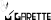
\includegraphics[width=0.33\textwidth]{cigarette.pdf}
\captionsetup{labelformat=empty}
\caption[Idéotexte de la \autonym{cigarette}]{}
\end{figure}
\poemtitle{La boisson}
\begin{verse}
Geste au combien cinématographique\\
Qui du briquet n’envie pas l’esthétique.\\
Saisissant la tasse à la belle croupe,\\
C’est aux cieux que je lève cette coupe.\\
Pour l’élégance, je porte à la lèvre avide\\
Mon verre de café depuis bien longtemps vide.
\end{verse}

\poemtitle{De l’attablée}
\begin{verse}
Assise au café,\\
C’était elle la boisson\\
Que je sirotais.
\end{verse}

%\paragraph{}
\begin{prose}
Là, je fis une rencontre, assurément des plus charmantes, celle de mademoiselle F*****.
\end{prose}



\poemtitle{Bout des doigts}
\begin{verse}
Lorsqu’à peine de ses doigts elle m’effleure.\\
Ô nuit, ô yeux, ô yeux, ô nuit\endnotemark[\getrefnumber{foot.vocaliseYeuxNuit}]\\
C’est une pluie qui ravit par sa fraîcheur.
\end{verse}

\begin{figure}[h]
\centering
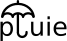
\includegraphics[width=0.33\textwidth]{pluie.pdf}
\captionsetup{labelformat=empty}
\caption[Idéotexte de la \autonym{pluie}]{}
\end{figure}

\poemtitle{Clausewitz sur la redoute}
\begin{verse}
Te croyais-tu sur la redoute\endnote{Allusion à la redoute Raïevski dans laquelle se trouvait le général Clausewitz d’après ses écrits lors de la bataille de la Moskova—Borodino.} si malin ?\\
Clausewitz, je  dis à ta destination :\\
La guerre n’est que la continuation\\
De l’amour par d’autres moyens.\endnote{Allusion à la maxime phare de l’analyse clausewitzienne \enquote{La guerre n’est que la continuation de la politique par d’autres moyens} dans son ouvrage \work{De la guerre}.}

Était-ce pour de la politique qu’Ulysse\\
Mit à profit  l’immensité de sa métis\endnote{Qualité relative à l’intelligence sociale attribuée à Ulysse. À raprocher de la ruse.},\\
Et que tous les Achéens\endnote{Les Grecs, énemis des Troyens.} périrent en lice ?\\
Ou bien était-ce pour ravir Hélène à Pâris ?
\end{verse}

\poemtitle{Battement de lèvres}
\begin{verse}
Zygène étend ses deux ailes\\
Prête à s’envoler\\
N’était qu’un sourire.
\end{verse}

\poemtitle{Fruits rouges}
\begin{verse}
Myrtille, framboise, fruit de la passion,\\
Dégustons les délices de l’instant de braise.\\
Sans le moindre égard pour tous les qu’en-dira-t-on,\\
Nous croquerons bien encore cerise et fraise.
\end{verse}

\poemtitle{Le trait}
\begin{verse}
Elle se retourna dans un furtif regard\\
Que vite je saisi dans l’instant subreptice\\
En l’assassinant d’un de mes traits qui égarent\\
Mais qui ricochât sur son œil plein de malices.

À peine les flèches eurent-elles sifflé,\\
Que déjà dans le tronc d’arbre elles sont fichées.\\
Et tel la grise fumée  qui suit  l’incendie,\\
L’ultime bourdonnement enfin s’entendit.

Et des cercles concentriques de sa pupille\\
Que l’on crut cible mais qui se révèle archère,\\
Parti la verbération qui fendit l’air\\
Et c’est dans mon cœur que le bourdonnement s’ouie.
\end{verse}



\poemtitle{De l’heureux jardin}
\begin{verse}
Au jardin heureux,\\
Par dessus le tapis  vert,\\
S’étend le ciel bleu.
\end{verse}

\poemtitle{Noces macabres d’Antigone et Hémon}
\begin{verse}
En criant emmurée dans la grotte, l’âme en\\
Peine, tu attire cependant ton amant.\\
Et celui qui accourt vers toi tel un aimant,\\
Pour se joindre à ta mort, celui-là est Hémon.

Le lit nuptial se sculpte dans le tombeau\\
Là où l’hymen ne sera jamais en lambeau,\\
Et ce que noue Vénus survivra aux enfers\\
Car Hadès, lui même, ne saurait le défaire.
\end{verse}

\poemtitle{Récollection}
\begin{verse}
Nous aimons nos morts, nous louons leur mémoire,\\
Et les chérissons bien plus que les vivants\\
Sans doute est-ce parce que bien moins souvent\\
Ont-ils l’occasion de nous décevoir.
\end{verse}

\poemtitle{Le secrêt}
\begin{verse}
Ce qui n’a pas su être dit,\\
Ce qui ne le sera jamais,\\
C’est dans l’ombre qu’il s’y ouïe\\
Et s’en entendent les méfaits.
\end{verse}

%\paragraph{}
\begin{prose}
Je promis à F***** de venir la voir à Eljadida dès après \fallbackserif{Ȝ}īd al\,Aḋĥā.
\end{prose}

\begin{prose}
Mais pour l’instant, sous les murailles de la vieille ville de Salé, m’apparurent de jeunes filles qui quoiqu’emmitouflées dans des ĥaïks, n’en demeuraient pas moins coquette avec leurs vêtements contemporains en dessous. D’improbables chaussures à talons aux couleurs vives pointaient même… un clapsus faillit me faire écrire \enquote{piédestal}.
\end{prose}

\poemtitle[ln(3) la plus belle de toutes]{\mathversion{bold}$\ln{3} $\mathversion{normal} la plus belle de toutes}
\begin{verse}
Personne ne sait ce qui se passa,\\
À la suite de la guerre de Troie\\
Mais je vais vous le dire sans  débattre\\
Ce qui eu lieux, c’est la guerre de Quatre.
\end{verse}


\begin{figure}[h]
\centering
\includegraphics[width=0.30\textwidth]{chellah.pdf}
\captionsetup{labelformat=empty}
\caption[Idéotexte du \autonym{Chellah} (\textarabic{شالة})]{}
\end{figure}


%\afterpage{
%\thispagestyle{empty}
%\AddToShipoutPictureFG*{%
%  \AtPageLowerLeft{\input{img/haik-pleine-page.pdf_tex}}
%}
%%\end{figure}
%~
%\vfill
%\pagebreak
%}

%\afterpage{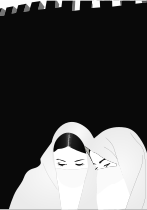
\includepdf[pages={1},addtolist={1,figure,{Dames au ĥaïk},haik}]{haik-monochrome.pdf}}

%\afterpage{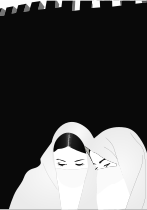
\includepdf[pages={1},addtolist={1,figure,{Dames au ĥaïk},haik}]{haik-monochrome.pdf}}
%\poemtitle{Ĥaïk}
%\begin{verse}
%Soutenant du dessus du blanc litham\endnote{Bande d’étoffe couvrant la partie basse du visage des femmes, juste en dessous des yeux.}\label{foot.litham}\\
%%\clearpage % TEMPORAIRE
%Un regard insolent de peccadille.\\
%Mystère du tissus qui déshabille\\
%Davantage qu’il ne vêtit les femmes.
%
%Triangle facial de chaire blanche\\
%Au haut pyramidion capillaire\\
%Est peau de chagrin pleine de lumière\\
%Où s’agrippent de lestes espérances.
%
%Cette obscénité qui se fit pudeur\\
%Serti le visage décolleté,\\
%Et à l’endroit où l’on retient l’ardeur\\
%Crée une si nouvelle nudité
%
%Où la pupille qui pointe en téton,\\
%Aréolée de khôl. Quand il se baisse,\\
%Soustrait aux regards ses délicatesses,\\
%Opposant des sourcils en un auvent.
%
%Et sourcils effilés jusqu’au canthus,\\
%En un ongle lacérant ma poitrine\\
%Qui est alors l’âtre ou siège chagrine\\
%La flamme aux feuilles tissées de lotus.
%
%Resplendissants et glorieux visages,\\
%Pistils des femmes emplis de présages\\
%Aux cheveux sépales qu’elles cajolent,\\
%Se sont-ils adjoint pareilles corolles ?
%\end{verse}


\poemtitle{La fleure}
\begin{verse}
M’enlisant dans le lieux commun\\
Que tous les scribouillards crétins\\
Ont épuisé jusqu’à l’écœurement\\
Je prétend en faire un ravissement

Car la Fleur que je ne peux emporter\\
Je l’admire  sans pouvoir la cueillir\\
Et si l’étreinte,  la ferait périr\\
Gérard de Nerval, saura m’excuser.
\end{verse}


\poemtitle{Des cliquetis}

\begin{verse}
Cliquetis claudiquent\\
Sur le cadran métallique\\
Avec conséquence.
\end{verse}

\begin{prose}
J’écrivis ce poème sous l’influence de la figure de Lissān~al\,Ḋḋīne ibn~al\,Xatīb et particulièrement de son muwacaĥ \work{Jadaka al-ṙaytu} que je venais de découvrir à la faveur d’un enthousiasme naissant pour la faste période d’al~Andalous et de l’intérêt impérieux que j’en nourris encore. Il me sembla que certaines associations, tournures et images qui, sans doute, n’influencèrent pas littérature française contrairement à d’autres œuvres arabes, méritaient d’être filées et ciselées encore. Je ne pu alors résister à la puissance des images qui fleurissent dans ses poèmes, à l’écoute desquels un oud se met entre mes mains et me voilà assis sur le rebord d’une fenêtre de l’Alhambra à contempler l’immensité de la péninsule hibérique conquise aux Goths. De Tariq ibn~Ziyyād à la Reconquista, mais bien au delà à travers l’influence qu’eu cette partie de Dar al\,Islam sur les troubadours, c’est toute al~Andalous que je tient d’un seul tenant. Et alors abu\,\fallbackserif{Ȝ}ab~Allah Mohammad {I}\ier{} ne croyait pas si bien dire, \xenism{Wa lā ṙāliba illā-llāh}, \enquote{Et il n’y a de vainqueur qu’Allah}.

%Quoique la chose ne fût pas au départ volontaire, mais finit par s’imposer, une métaphore filée du thème de l’astronomie traverse cet écrit.
\end{prose}

\poemtitle{L’horizon élégiaque}
\begin{verse}
Enrobé dans la noirceur ordinaire,\\
De mes nuits si longues et solitaires,\\
Je béni celui-là qui des transports\\
N’en sait davantage que Guethenoc.\\
Toi, le paysan accablé d’efforts\\
Qu’en cette matière tu reste sot,\\
Que dans une ignorance bienheureuse,\\
Tu côtoie la stase délicieuse\\
Celle-là qui me sera étrangère\\
Comme elle le fût si souvent naguère.

Car bien plus familier m’est le crépuscule\\
Depuis que ces attraits, de mes littoraux,\\
Ne s’en sont approchés par un vil recul\\
Sans amarre, que pour mieux s’y dérober,\\
Me laissant dans un pareil dépouillement\\
Et qui me frustre jusqu’aux points cardinaux.\\
J’ouvrirais tous les ports à ces sentiments,\\
Malgré la défaveur de l’amirauté. 

Peut de choses je pourrais rapporter\\
Du ravissement où ils me laissèrent,\\
Sinon des bribes qui, quoiqu’oubliées\\
Font chanter les nations de concert,\\
Un évangile qui ne peut s’exposer\\
Ni ici sur terre ni haut dans les airs. 

Un brasier rendit mon âme bien frêle\\
Près duquel le soleil n’est qu’étincelle\\
Car du voluptueux dandinement,\\
Paraissent de subreptices croissants\\
Dont la lune, de ses librations,\\
Ne peut que jalouser l’inflation.\\
Trois dimensions est une bonté\\
Que nous accorda la Divinité\\
Pour que les corps et leur rotondité\\
Puissent à tout loisir de se cuber. %TODO faute

Elle qui sans pétales, dévoile un pistil,\\
Dont la parjure clarté transperce la nuit,\\
Mais que l’on cache par des procédés habiles,\\
Fait danser son élégante tige qui fuie\\
Dans une fort captivante nyctinastie.\\
Sous ma vive acclamation de spectateur,\\
Au galant de nuit et sa fanfare olfactive,\\
Qui à la tombée du jour promptement s’active,\\
Ma sueur s’est vite mêlée à la senteur.

La parhélie étrangère à nos contrées\\
Rend le vaste horizon insignifiant\\
Et peu me chaud d’en distinguer\\
Son orient, de l’occident.\\
Mes yeux ne se poseront plus que sur les sien,\\
Puissè-je me suffire d’un millénaire\\
Pour parcourir et le mal et le bien\\
De cette distance pupillaire.%
%
\endnote{%
Aux quatre derniers vers de cette strophe qui ont une métrique dégressive en 12--11--10--9, existe une variante isométrique en alexandrin :%
\begin{verse}%
Mes yeux ne se poseront plus que sur les siens,\\
Puissè-je me suffire d’un seul millénaire\\%
Pour parcourir l’étendue  du mal et du bien\\%
Jonchant cette infinie distance pupillaire.\\%
\end{verse}%
}

Faut-il filer à pareille allure, ô temps ?\\
Veuilles atténuer mon affliction\\
En ralentissant l’irrévocable cours,\\
Que je m’adonne à la contemplation,\\
Que j’en fixe quelques suaves contours.

Fasse du sablier clepsydre\\
Emplie de l’âme qui me plut.\\
Étanche mon inclination.\\
Lorsque gronde l’incendie ardent\\
Même lorsque frappé par le vent,\\
Celui qui est de l’éloignement,\\
Il brûle et puis s’accroît jusqu’aux nues.

Maudit été, au solstice duquel\\
Je veux tordre l’odieux nocturlabe.\\
Vive les longues nuits avec la belle\\
Où se fait leste le contour du galbe. 

Lune et soleil sous sa gorge nue,\\
Et dans sa pupille, en logarithme,\\
Se projette l’univers connu,\\
Dont le mouvement stellaire en rythme\\
Cache des galaxies au nikab.\\
Peu m’importe qu’on puisse médire,\\
Pour la voir du zénith au nadir,\\
Je délaisserais les astrolabes.

Que Dieu et les hommes soient témoins\\
Des larmes  que j’ai souvent versés,\\
Si denses que le soir en est oint,\\
Le ciel nocturne en est constellé.\\
Épanchées du fait de son l’absence\\
Elles remplissent une tasse de café\\
Qui a les anneaux de saturne pour anse.
\end{verse}

\begin{figure}[h]
\centering
\includegraphics[width=0.7\textwidth]{saturne.pdf}
\captionsetup{labelformat=empty}
\caption[Idéotexte de \autonym{Saturne}]{}
\end{figure}


\poemtitle{Crépuscule écarlate}
\begin{verse}
Laps. Le samurai,\\
Rengainant son katana,\\
Mit les nues à sang.
\end{verse}

\poemtitle{Nohimé}
\begin{verse}
Nohimé,\\
Ton nom est sur les murs gravé,\\
Nohimé,\\
Ô terrible Nohimé,\\
Il le sera à jamais.

Nohimé,\\
Et il l’est par le sans versé\\
Celui qui coagulait.

Nohimé,\\
C’est le prix de l’éternité\\
Et tu t’en ai acquittée.

Nohimé\\
Ton nom est toujours évoqué.\\
Même loin de ta contrée,\\
Malgré l’ancienneté.\\
Nohimé.
\end{verse}

\poemtitle{Délire}
\begin{verse}
Au sommeil pesant,\\
Nuée de corbeaux s’envole\\
N’était que mes cils.
\end{verse}

\poemtitle{Point d’insomnie}
\begin{verse}
Poussé jusqu’au pied de mon lit\\
Par une rêverie folle,\\
Je me retrouvai au sol\\
Comme le point tombé de l’ı.
\end{verse}

\poemtitle{La momie péruvienne}
\begin{verse}
Elle pétrifie autant qu’elle est figée,\\
Ses mains sont liées mais elle nous saisit.\\
D’effroi alors, car ses traits sont affligés.\\
Elle nous regarde nous, êtres livides,\\
Adressant un cris muet qui dessaisit,\\
Elle nous regarde de ses globes vides.

Ceignant la mort en position fœtale,\\
Comme le nouveau-né qui vient à la vie\\
Et délivrant par le trou occipital,\\
Un seul message à jamais inassouvi.

Que veut-elle nous dire du fond des âges ?\\
Que veut-elle  de nous par delà la mort ?\\
Ses grands yeux noirs nous semblent insoutenables\\
Quand ils nous cachent un mystère insondable,\\
Terrifiants parce qu’emplis de remords,\\
Nous en comprenons peut-être le message.

Ce qui suscite la crainte et la torpeur\\
Est que le repos n’est guère dans la mort\\
Alors donc dis-nous tout, sans crainte ni peur.\\
Momie, nous écoutons ton cris insonore.
\end{verse}

\section*{Forêt}
\markboth{}{Forêt}
\addcontentsline{toc}{section}{Forêt}
\poemtitle{Du Gévaudan}
\begin{verse}
Des crocs scintillants\\
De la Bête menaçante,\\
La vallée de larmes.
\end{verse}

%\begin{prose}
%Je me rendis à la forêt de Mamora, non loin de Kénitra où je pu m’exercer à l’arc, peut avant \fallbackserif{Ȝ}īd al\,Aḋĥā.
%\end{prose}

\poemtitle{Une forêt pour mille ans}
\begin{verse}
Voici notre legs à la postérité\\
Qui verra majestueux les pouces plantés\\
Lorsqu’ayant atteint la hauteur impériale.\\
Et l’on en verra la canopée des étoiles.

Que soient  témoins les arbres qu’ici nous plantons,\\
Que la décennie n’en soit que le liminaire,\\
Que dans un siècle on dise encore \enquote{Il y’a cent ans},\\
Que dans mille ans on commémore un millénaire.
\end{verse}

\poemtitle{L’archer forestier}
\begin{verse}
Ricoche brutale flèche d’airain,\\
Sur la roche solide du sapin,\\
Comme le boulet de l’artillerie,\\
Qui sur la fière tour  ronde dévie.\endnote{En architecture militaire médiévale, les tours à base ronde sont connues pour être plus résistantes, notamment face au tirs d’artillerie, que les tours à base carrée.}\label{foot.tourRonde}

Mais de sève de Salicacées saturée\\
Enfonces-toi dans l’essence du peuplier\\
Qui au retour en laisse la pointe souillée\\
Et âcre d’une jaunâtre viscosité.

Si les arbres ne peuvent nous contenter,\\
Tournons-nous alors et pointons le palmier\\
Dont le stipe amoureux accueille d’égards\\
Quoique, jaloux, retient fermement le dard.

Reste donc le chêne-liège doux de bois\\
Qui, quoique par cette saison démasclé,\\
Est la  cible dont le tissage parfait\\
Prend la flèche et me laisse la retirer.
\end{verse}

\poemtitle{Lendemain de bataille}
\begin{verse}
Faire couler tant de sang,\\
En fertiliser le sol,\\
Et s’y oindre abondamment.\\
Rien d’autre ne me console.

Oui, le sang dont on se fard\\
Sur les champs où sont tombés\\
Les corps que j’ai enjambés\\
Et qui n’est alors qu’essart.

En compagne effarouchée,\\
La guerre les a couchés\\
Dans son lit d’éternité,\\
Me jetant sa vanité.

L’amertume bien trop longue\\
Y a un goût métallique\\
Qui, écarlate et publique,\\
Pique le bout de la langue.

Plus rien n’y est vertical,\\
Si ce n’est quelques chacals\\
Et l’épée dont le pommeau\\
Sert de perchoir au corbeau.
\end{verse}

\poemtitle{Du komorebi}
\begin{verse}
Branches de forêt,\\
Le soleil sait s’y frayer\\
D’inattendus gués.\endnote{Le \xenism{komorebi} est dans la culture japonaise, le phénomène visuel par lequel les rayons du soleil se faufilent à travers les branches des arbres.}
\end{verse}

\poemtitle[Na Trioblóidi]{Na Trioblóidi\endnote{Nom en gaélique irlandais donné aux \enquote{Troubles}, c’est à dire le conflit nord-irlandais qui a ensanglanté l’Irlande des années 1960 aux années 1990.}}
\begin{verse}
Depuis que débarqua Oliver Cromwel\endnote{La domination anglaise sur l’Irlande fut rétablie à partir du débarquement d’Oliver \textsc{Cromwel} sur l’île où il instaura des lois pénales discriminatoires envers les catholiques.},\\
Sur ton rivage, avec sa New Model Army\endnote{Armée de la Première révolution anglaise qui a été organisée et formée par \textsc{Cromwel} sur le modèle de ses propres troupes.}\\
Tu tiens toujours au nord comme à ta prunelle\endnote{Encore aujourd’hui, le nord de l’île est occupé par le Royaume-Uni.}\\
quelque soient les infamies de l’ennemi.

Avec ses bombes, et ses tanks et ses drones\endnote{Allusion au refrain de \work{Zombie} des Cramberries puissamment chantée par la regrettée Dolores \textsc{O’Riordan} au sujet du traumatisme du conflit nord-irlandais et qui dit :
\begin{verse}
With their tanks, and their bombs\\
And their bombs, and their guns
\end{verse}
}\\
Il croit te tendre la main comme une sœur\\
Mais c’est une infâme traîtrise du Trône\\
Qui tient la main droite rouge de l’Ulster\endnote{L’Ulster est une région historique de l’Irlande qui coïncide plus ou moins bien avec l’Irlande-du-Nord qui est l’entité sous domination britannique. La main droite ensanglantée en est le symbole héraldique traditionnel.}

Mais lorsqu’il s’en ira,\\
Nous tous l’on en rira.\\
Le poitín\endnote{Boisson traditionnelle irlandaise.} jaillira,\\
Et vainqueurs l’on boira\\
Car partout l’on dira\\
Son règne périra.
\end{verse}

\poemtitle{La confidente du jour}
\begin{verse}
Elle arrivait face au jour et sa clarté,\\
Emplie d’une gaieté annonçant l’été\\
Qui accueil le ciel et sa luminescence,\\
Pour se gorger de pleine réjouissance.\\
Les commissures de ses lèvres vermeil\\
Étaient bien retroussées jusqu’à ses oreilles\\
Comme une leste archère ayant l’arc bandé\\
Auquel est encoché la joie débridée.\\
C’était sur elle que la joie scintillait,\\
Mais c’était le soleil qui lui souriait.
\end{verse}

\poemtitle{De l’abeille}
\begin{verse}
L’abeille grappille.\\
Posée sur la camomille\\
Est grain de beauté.
\end{verse}

\begin{figure}[h]
\centering
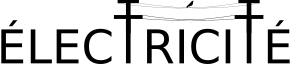
\includegraphics[width=0.6\textwidth]{electricite.pdf}
\captionsetup{labelformat=empty}
\caption[Idéotexte de l’\autonym{électricité}]{}
\end{figure}

\poemtitle{Sous les néons de la nuit}
\begin{verse}
Sous les néons du lampadaire,\\
Je suis debout et solitaire.\\
Et sur la flaque, singulières\\
S’éclaboussent tant de lumières.

Là, les gouttelettes de l’éclairage\\
Se diffractent en nombreux clapotis \\
Qui dans cette rue sont l’unique bruit.\\
Elles ne semblent être qu’un mirage.

Voile de silence que cette pluie\\
Abattue sur la noirceur de la nuit\\
Que franchi la ligne phosphorescente\\
De la moto que Mokoto pilote.

Aussitôt suivit par de vives traînes\\
Que la persistance rétinienne\\
Conserve encore dans ma pupille\\
Enfourchant ma moto, je les suis.
\end{verse}


\poemtitle{Fleur d’engrenage}
\begin{verse}
Tu perds tes pétales sur les chaînes d’assemblage\\
Où fuie ta jeunesse, toi la fleure d’engrenage.

Kilomètres de câblage ont meurtri tes épaules\\
Qui, endolories,  sont des sépales sans corolles.

Sur la liane en métal, se brise ton jeûne âge\\
Car pour l’industrie, tu es la fleure d’engrenage.

Parce que l’on te sait belle mais fragile,\\
Les quolibets te trouvent cible facile.

N’est-ce pas le bourdon qui prétend manager\\
Qui vient, tout velu, à ta tige se frotter ?

Oppose à la peine et au commérages\\
Tes six épines de fleur d’engrenage.

L’on te méprise et dédaigne, fille du câblage,\\
Mais au verger, tu es l’unique fleur d’engrenage.

Celle que je veux arroser de richesses,\\
Et la seule que je comble de tendresses.

Qu’à jamais se dessine la fierté\\
Sur les trait des visages ouvriers,

De celles qui sont plus belles que les bourgeoises.\\
Vous qui êtes d’éclatantes fleurs d’engrenages.
\end{verse}

%\begin{figure}[h] % TODO
%\centering
%\includegraphics[width=0.3\textwidth]{hofra.pdf}
%\captionsetup{labelformat=empty}
%\caption[Idéotexte du \autonym{trou} (\textarabic{حفره})]{}
%\end{figure}

\poemtitle{Astres nourriciers}
\begin{verse}
Sous sa gorge qui émerveille,\\
Luisent la lune et le soleil.
\end{verse}

\poemtitle{Caresses de l’oud}
\begin{verse}
À la première caresse de l’oud,\\
L’onde me fait trembler du bras au coude.\\
Si ma respiration s’amenuise,\\
Aucune autre émotion n’est permise.
\end{verse}

\begin{figure}[h]
\centering
\includegraphics[width=0.30\textwidth]{adm-3a.pdf}
\captionsetup{labelformat=empty}
\caption[Terminal ADM-3A]{}
\end{figure}




\poemtitle{Boucles de cheveux}
\begin{verse}
Les boucles qui encadrent son visage,\\
Comme autant de volutes de violon,\\
Font une si jolie chanson, en présage\\
De la caresse de nos doigts fêlons.
\end{verse}

\poemtitle{Ode du programmeur}
\begin{verse}
Dans la douce noirceur de la nuit\\
Les gouttelettes typographiques\endnote{La \enquote{pluie de caractère} est un motif ésthétique emprunté à \work{La Matrice}.}\\
Ruissellent au delà de minuit\\
Sur mon terminal panoramique

Et les méthodes\endnote{En programmation informatique, les méthodes sont des fonctionnalités qui s’appliquent à certains objets. Une méthode pouvant elle même avoir d’autres méthodes. Dans certains langages de programmation, l’appel à une méthode sur un objet se fait en arrimant cette méthode à l’objet. Par exemple, sur l’objet \texttt{objet} s’applique la méthode \texttt{méthode} de la façon suivante : \texttt{objet.méthode}. Si une seconde méthode \texttt{méthode2} devait s’appliquer sur l’ensemble, celà prendrait la forme \texttt{objet.méthode.méthode2}.} s’enchaînent et s’arriment\\
Tel des wagons qui s’avancent dans le soir\\
Jusqu’à ce qu’une erreur ne vienne surseoir\\
À la course du codeur pusillanime.
\end{verse}

%\afterpage{
\includepdf[pages={1},addtolist={1,figure,{Le corps de la danseuse},corpsdanseuse}]{danseuse.pdf}}
%\afterpage{
\newpage{}
\thispagestyle{empty}
\AddToShipoutPictureFG*

\section*{Intermède}
\markboth{}{Intermède}
\addcontentsline{toc}{section}{Intermède}

%\poemtitle{Fleur d’Afrique}
%\begin{verse}
%C’est une magnifique fleure de lotus\\
%Qui traverse l’Afrique en un sillage vert\\
%Dont la tige serpente le long du désert\\
%Ainsi que l’encre coule sur le papyrus.
%
%Le Fayoum qui en est la feuille bourgeonnante\\
%Annonce le delta dont les eaux ondoyantes\\
%Forment la corolle, sans plus aucun laïus.\\
%Ou est-ce là un pétulant mont de Vénus ?
%
%Draine le limon,\\
%Ô fleure rebelle\\
%Là où nous buvons\\
%Tes eaux éternelles.
%
%J’ai vu dans le flot de tes eaux\\
%Le reflet du vol du faucon\\
%Emportant et le renouveau\\
%Et la chute des nations.
%\end{verse}

%\begin{floatpoem}
%\afterpage{
%\newgeometry{left=1cm}
%  \newgeometry{left=1cm, right=1cm, top=1cm, bottom=1cm}%
%\placetextbox{35}{190}{
%\poemtitle{Fleur d’Afrique}
%\centering
%\includegraphics[height=\textheight+2cm]{nil.pdf}
%}
%\restoregeometry
%}

%\afterpage{
%  \newgeometry{left=1cm}
%  \begin{figure}
%  \includegraphics[height=\textheight-1cm]{nil.pdf}
%  \end{figure}
%AFTERPAGE

%\placetextbox{35}{190}{
%%\poemtitle{Fleur d’Afrique}
%\centering
%\includegraphics[height=\textheight+2cm]{nil.pdf}
%}
% \afterpage{
% \restoregeometry
% }
%}

%\end{floatpoem}
\poemtitle{Clapotis de l’averse}
\begin{verse}
Avec clapotis,\\
De l’inopinée averse,\\
L’espoir se déverse.
\end{verse}


\begin{prose}
Avant \fallbackserif{Ȝ}īd al\,Aḋĥā, j’eu le plaisir de rencontrer une jeune femme que je vis d’abord, chose rare, sous son litham. Je dois admettre que ce vêtement censé repousser m’attira en réalité. Elle m’accorda même l’honneur de m’entretenir si bien que nous pûmes découvrir notre passion commune pour l’ouvre de fiction de Frank \textsc{Herbert}. Fait notable, lorsqu’elle retira son voile, je vis qu’elle avait des points de rousseur qui me rappelèrent le \enquote{gout de cannelle} qu’a l’épice récoltée sur Dune.
\end{prose}

\poemtitle{Litham}
\begin{verse}
Litham\endnotemark[\getrefnumber{foot.litham}], haute muraille aux merlons de dentelle.\\
D’un créneau se manifesta l’archer rebelle.\\
De la belle, il est l’aiguisée pupille noire\\
Qui darde l’œil et est cible de mon regard.

D’une fugace œillade, une seule, elle encoche\\
Et d’un battement de paupière elle décoche.\\
Toi qui de la vertu est la protection,\\
Tu accroît sa vulnérabilité, pourtant.
\end{verse}



\begin{prose}
Et je composais alors sans doute mon première poème en arabe littéral dont je vous donnes ici la traduction qui, fatalement, sacrifie la métrique autant que les rîmes.
\end{prose}

\begin{longtable}{R{0.3\textwidth} L{0.65\textwidth}}

\noalign{\vspace{-0.5cm}\poemtitle[Dune d’Arrakis — \textarabic{كثيب أراكيس}]{\textarabic{كثيب أراكيس} — Dune d’Arrakis}}
\endfirsthead

\textarabic{هيبتها الأبدية}		& Son éminence éternelle\endnote{Dans l’œuvre de fiction de Frank \textsc{Herbert}, Arrakis est une planète désertique aussi appelée par ses autochtones \autonym{Dune}.}\label{foot.DuneArrakis}\\
\textarabic{ترشدنا في الخلاء}		& Nous guide dans la vacuité\\
\\
\textarabic{و عمرها لا يحصا}		& Elle est sans âge\\
\textarabic{لما تملأنا بالهناء.}		& Lorsqu’elle nous emplit de joie.\\
\\
\textarabic{لكل من راء الرمال دائم،}	& À quiconque aura vu les sables perpétuels,\\
\textarabic{هيا مقام الصحراء.}		& Elle est l’espar du désert.\\
\\
\textarabic{من تحت الهلالين،}		& D’en dessous des deux lunes\endnote{Autour de la planète Arrakis orbitent deux satellites naturels.},\\
\textarabic{منحنياتها تطربنا.}		& Ses courbes nous ravissent.\\
\\
\textarabic{يا روعه الكثبان،}		& Ô magnificence des dunes,\\
\textarabic{بسموّك أملينا،}		& Empli-nous de ton excellence,\\
\\
\textarabic{امنحنا التسامي،}		& Dote-nous de sublimation,\\
\textarabic{بالمجد شسب عطشنا.}		& Étanche notre soif de gloire.\\
\\
\textarabic{و الدنيا أعلنت}		& Et l’univers a déclaré\\
\textarabic{﴿من زارها زارني﴾.}		& \enquote{Qui l’aura visité m’aura visité}\endnote{La planète Dune est un lieux de pèlerinage.}.\\
\\
\textarabic{بفضل متعتك،}			& De la jouissance qui émane de toi,\\
\textarabic{ازرقت اعيني.}		& Mes yeux bleuirent\endnote{L’atmosphère de Dune est saturée d’une substance appelée épice qui a de nombreux effets métaboliques sur le corps humain dont celui de rendre les yeux bleu ce que l’on nome le regard de l’\autonym{ibad}.}\label{foot.regardibad}.\\
\\
\textarabic{في خطوط المستقبل،}		& Dans les lignes de l’avenir,\\
\textarabic{رأيت باطمئنان}		& J’ai vu avec quiétude.\\
\\
\textarabic{كل العقود الخبيته}		& Tous les nexus néfastes\\
\textarabic{نفيت في مهب الرياح.}		& Furent emportés par les vents.\\
\\
\textarabic{في مجاري الزمان،}		& Dans les couloirs du temps,\\
\textarabic{تقدمنا و تراجعنا.}		& Nous avançâmes et reculâmes.\\
\\
\textarabic{حتى فتح الممر،}		& Jusqu’à ce que se soit ouvert le passage,\\
\textarabic{ركضنا مبتهجون.}		& Nous avons galopé euphoriques.\\
\\
\textarabic{تقيضنا نحوا الهدى،}		& Tu nous guide vers le sentier,\\
\textarabic{الهدى الذهبية.}		& Le sentier pavé d’or.\\
\end{longtable}

\poemtitle{Pommettes}
\begin{verse}
Pommettes qui font rayonner la joie,\\
De pulpe de pêche, elles sont gorgées.\\
Les rayons d’or s’y sont éclaboussés\\
Et la rosée en fait encore foi.
\end{verse}



%  \newgeometry{left=1cm, right=1cm}
%  \begin{figure}
%  \includegraphics[height=\textheight-1cm]{nil.pdf}
%  \end{figure}
%  \restoregeometry

\poemtitle{Le voile et le suaire}
\begin{verse}
Maudit soit celui qui avec quelques haillons\\
Voudrait dérober cette œuvre à nos sentiments.\\
Elle ne sera ôtée de notre visière\\
Que lorsqu’enfin enveloppée dans le suaire.\\
\end{verse}


\poemtitle{Andalousie, toujours}
\begin{verse}
Dans les nuits dont la noirceur drapait nos transports\\
Nous humions les effluves du jasmin nocturne\\
Tandis que les étoiles emplissaient nos verres,\\
Celles que le soleil du matin évapore\\
Et avec elles, ce qui fit notre fortune\\
Avant que ne nous ai séparé le désert.
\end{verse}


\poemtitle{Pyrogenesis}
\begin{verse}
Comme un vieux destrier qui s’en va pâturer,\\
Et qui clôt les yeux dont s’épanchent quelques larmes,\\
Débarquent de sous mes paupières armurées\\
Les nefs, les engins de siège, et le peuple en arme.

Eux qui sortent des casernes et forteresses\\
Fourmillent sur le territoire pour s’étendre,\\
Sacrifiant à la guerre et à son ivresse,\\
Le sang de chaque ennemi qu’ils s’en vont répandre.

Ils encerclent à mes ordres les bâtiments\\
Prennent les édifices, pillent les ressources ;\\
Nourriture, bois, pierre, métal et eau douce,\\
Sous les râles des humains et les bêlements.

Ces images qui persistent à me hanter\\
À chaque  fois que me saisit une somnolence,\\
Avec les tambours de guerre au timbre argenté\\
Sentent l’odeur de la mort et sa pestilence.

Car si je séduisis la belle Cléopatre,\\
Et réduisis en cendre sur le Nil albâtre\\
Les trirèmes britons des légions romaines\\
Qui tinrent garnison sur les plateaux et plaines,

Sur l’isthme de Corinthe je les contins,\\
Eux les Gaulois qui arrivent du lointain.\\
Tandis que les commerçants d’Anatolie\\
Apportaient poterie et dinanderie.

Exploitant les mines de fer et  les forêts,\\
J’ai épuisé les ressources et les denrées\\
Et c’est ainsi que j’atteignis le troisième âge\\
Dont les merveilles érigées font témoignage.

Dans la savane, en Asie, ou sur les Cyclades\\
Devant les pylônes ou au pied des montagnes,\\
Je commande au peuple qui toujours m’accompagne\\
Femmes, paysans, fantassins par myriades.

Je fis cela et plus encore, vous dis-je\\
Je fis tout cela, et je battis  des records\\
En témoignera même le tableau  des scores\\
Car mes hauts faits n’auront jamais été qu’un jeu.
\end{verse}

\poemtitle{Arôme acre}
\begin{verse}
Quand le café coule dans ma gorge,\\
Je le sens ruisseler sur la tienne,\\
En épouser les formes troyennes\\
Et les beautés dont elles regorgent.
\end{verse}

\poemtitle{La surfeuse}
\begin{verse}
M’avisant, adossée au ciel,\\
Sont-ce les boucles du soleil\\
Ou les rayons de ses cheveux\\
Qui volent en mèches de feu ?
\end{verse}

\poemtitle{Pattes de velours}
\begin{verse}
De son cou et de son pourtour,\\
Mes doigts  qui en tracent le contour\\
Sont des caresses d’araignée\\
Qui pose ses pattes de velours.
\end{verse}

\poemtitle{Les flots de la danseuse}
\begin{verse}
Au premier pincement du kanoun\endnotemark[\getrefnumber{foot.kanoun}],\\
De la corde part l’onde singulière\\
Jusqu’à mouvoir le corps de la corsaire\\
Qui, à l’abordage de mon âme, la détourne.

Accompagnant sa lascive danse,\\
Elle chante l’oraison funèbre\\
Qui scelle le trépas de mon innocence,\\
Et une passion secrète célèbre.

Et contrairement à l’Ithaquien\endnotemark[\getrefnumber{foot.ithaquien}],\\
Nul besoin de m’attacher au mat\\
Tant les charmes nouent le lien\\
Et que toute raison m’abandonna.

Navigant sur les courbes, ma flotte\\
À chaque port ravit les merveilles\\
Car de ce pays je suis l’oramanaute\endnote{Hapax. Du grec ὅραμα, \enquote{spéctacle} et du latin \xenism{nauta} \enquote{navigateur}. Pouvant être compris dans le sens d’\enquote{explorateur des beautés}.}\\
Qui vogue sur l’océan vermeille.

Mais d’une carte mouvante il faut me munir\\
Car la tectonique des côtes charnelles\\
Est d’une inconstance qui sait ébaudir\\
Par la souplesse que seule connait la belle.
\end{verse}





\poemtitle{Grains de beauté}
\begin{verse}
L’infini et l’infime se reflètent,\\
Dans cette poudre qui s’étiole.\\
Mais sont-ce étoiles ou lucioles\\
Que les grains de beauté sur ses pommettes ?
\end{verse}

\poemtitle{Du regard}
\begin{verse}
Ton regard sévère,\\
Je crains autan que j’espère\\
Qu’il ne me repère.
\end{verse}

\poemtitle{Les Amphores}
\begin{verse}
Vastes amphores, gloire de celle qui les tracte\\
Que, doubles, les belles abondances du Ciel firent\\
Et que le champs de vision ne peut contenir\\
Lorsque les cheveux lisses coulent en cataracte.

D’un minois gracieux et docile,\\
Heureuse, de sa croupe fertile,\\
Nous présenter l’offrande servile\\
Dans un mouvement leste et gracile.

Balançant souplement en arrière la tête,\\
Elle rejette d’aussi infinis cheveux\\
Que l’envergure déliée de sa gorge en feux,\\
Attendant que sa chemise soit donc défaite.

Le visage suave que parcourent les doigts\\
Dans une danse qui explore le moindre appas\\
Jusqu’aux lèvres sucrées dont la grande majesté\\
Ne dément certainement pas celle du fessier.

Maudit sois le galeux qui de quelques halons\\
Voudrait dérober à nos yeux ce monument\\
Car il ne sera ôté de notre visière\\
Hélas que  lorsqu’enveloppé par le suaire.
\end{verse}

\newpage
\newcommand\nildesc{\em 
}

\thispagestyle{empty}
%\newgeometry{top=1cm, bottom=1cm, inner=1.4cm, outer=0.3cm}

\AddToShipoutPictureBG*{%
  \AtPageLowerLeft{%
    \begin{tikzpicture}[remember picture]
      \node (nile)  at (current page.south west)
         {\hspace{3.2cm} \includegraphics{nil.pdf} };
      \node (B) at ([shift={(110:7)}]nile) {{\large\textbf{Fleur d’Afrique}%
        \addcontentsline{toc}{subsection}{Fleur d’Afrique}%
}};

      \node  at (current bounding box.south west) [anchor=south west]
        {
          \hspace{0.5cm}\begin{minipage}[t][14cm][t]{8.7cm}
            \shapepar{ 
{5}
{0}     b{0}\\
%
{0}     t{-1.0}{4.3}\\
{0.5}   t{-1.0}{5}\\
{1}     t{-1.0}{5}\\
{1.5}   t{-1.0}{4.7}\\
{6}     t{-1.0}{4.7}\\ % premier coude
{7}     t{-1.0}{6.4}\\ % premier coude
{8}     t{-1.0}{7.5}\\
%{10}    t{-1.0}{8}\\   % boucle
{10.7}    t{-1.0}{9.9}\\ % 
{11}    t{-1.0}{12.2}\\ % 
{11.5}  t{-1.0}{11.2}\\
{11.6}  t{-1.0}{11.2}\\
{12}    t{-1.0}{11.0}\\
{13}    t{-1.0}{11}\\
{14}    t{-1.0}{11.7}\\
{16}    t{-1.0}{12.4}\\ % centre de l’arc
{17}    t{-1.0}{12.0}\\
{18.5}  t{-1.0}{12.2}\\
{19}    t{-1.0}{12.3}\\
{19}    e{11}
            }%
            {\em Cette lassive \emph{fleur d'Afrique} décrit par sa tige le cours du Nil d'un point de vue zénithal tandis que le delta est figuré à la façon d'une corole de fleur de lotus selon sa représentation héraldique en Égypte antique. Et la région du Fayoum qui bourgeonne de cette fleur m'a semblé sur les photographies satellitaires en être la feuille, d'autant que son verdoiement ne laissait pas de doutes. J'avais tant de choses à dire au sujet de ce fleuve, au sujet de ce Fayoum notamment, qui me marqua autan que les portraits qui y furent retrouvés et dont il donna le nom à la série de portraits retrouvés ailleurs.  Ceux de ces personnes, parfois jeunes qui nous observent depuis le passé et surtout par delà la mort. On pourrait y lire un \emph{memento morri} et pourtant ils ont l'air incroyablement vivants, et j'oserais même dire contemporains. Ce sont des contemporains qui nous observent, des êtres qui auraient pu vivre en notre siècle et partager nos préoccupations. Tandis que tous reçurent un nom par les archéologues, m'intrigua alors plus encore que les autres, un portrait représentant une femme à laquelle l'historiographie ne semble pas en attribuer mais que j'appelle la dame aux sourcils noirs.}
          \end{minipage}
        };
      \node (other)  (current bounding box.south east) at ([shift={(30:7)}]nile) {
        \hspace{0.0cm}\begin{minipage}[t][7cm][t]{11cm}
\hspace{2.0cm}\textbf{\large Bataille d’Actium}%
\addcontentsline{toc}{subsection}{Bataille d’Actium}

\null\hspace{1.5cm}Nicopolis\endnote{Ville battie par Octave à la suite de sa victoire contre Marc-Antoine et Cléopâtre.}, cité de la victoire\\
\null\hspace{1.0cm}Trépas des amants\endnote{Marc-Antoine et Cléopatre~\textsc{vii}.} et de leur pacte,\\
\null\hspace{0.9cm}Qui se souvient encore de ta gloire\\
\null\hspace{0.8cm}Depuis le vif essor de Naupacte\endnote{Ville dont l’importance pirs le pas sur Nicopolis.} ?\\

\hspace{0.5cm}De qui célèbres-tu la victoire ?\\
\null\hspace{0.3cm}Est-ce de Cléopatre Philopator\\
\null\hspace{0.0cm}La belle qui est, osè-je croire,\\
\null\hspace{0.0cm}Plus que quiconque vivante dans la mort ?\\

\hspace{0.0cm}Si c’est Octave qui t’érigea en Épire,\\
\null\hspace{0.0cm}C’est Marc-Antoine et Cléopâtre qui vainquirent,\\
\null\hspace{0.0cm}Par leur amour si fructueux, ils nous conquirent.\\
\null\hspace{0.0cm}Loin d’en gâter la fécondité, le soupir\\
\null\hspace{0.5cm}En fit naître, non pas la défaite mais pire,\\
\null\hspace{1.0cm}Car en mourant, ils mirent au monde l’empire\endnote{À la suite de la mort des amants, et donc de la victoire d’Octave, Rome devint effectivement un empire.}.\\

\vspace{0.5cm}

\hspace{3.0cm}\textbf{\large Place de la Concorde}%
\addcontentsline{toc}{subsection}{Place de la Concorde}

\null\hspace{4.6cm}Nous prêtâmes sermon\\
\null\hspace{4.8cm}Sous les hiéroglyphes\\
\null\hspace{4.9cm}En est témoin le sang\\
\null\hspace{5.0cm}Apposé de nos griffes.

\vspace{0.5cm}

\hspace{4.7cm}\textbf{\large Larmichettes}
\addcontentsline{toc}{subsection}{Larmichettes}

\null\hspace{5.0cm}Sous la voilette,\\
\null\hspace{5.2cm}Trois gouttelettes\\
\null\hspace{5.3cm}Choient et s’arrêtent\\
\null\hspace{5.2cm}En vaguelettes\\
\null\hspace{5.1cm}Vers ses pommettes.



        \end{minipage}
      };

%       \node  at (current bounding box.south west) [anchor=south west]
%       {
%       };
%
%      \draw [red] (current bounding box.south east) rectangle (current bounding box.north west);
    \end{tikzpicture}
  }
}

\null
\newpage


\poemtitle{Le thé}
\begin{verse}
En le buvant, mes traits se font maussades.\\
On attend qu’il agresse le palais,\\
Qu’il m’émeuve ou fasse un quelconque effet\\
Mais il reste désespérément fade.

Qu’aux rameaux de menthe ou de camomille\\
Il soit mêlé, rien ne le bonifie.\\
Au thé, cette abominable fraude,\\
Je préfère  boire de l’eau chaude.
\end{verse}


\poemtitle{Rousseur}
\begin{verse}
Comme un met saupoudré de cinnamome,\\
On y souffla ennemie sans arôme.\\
Mais elle me laissa inconsolé\\
Car la cannelle s’était envolée.
\end{verse}

\poemtitle{Sourire de la rousse}
\begin{verse}
Semblable à la nuit idéale,\\
La rousse au visage satin\\
Paré de toutes ses étoiles\\
S’en vit dépouiller au matin\\
Quand, tel l’aurore, vint y luire\\
Un soleil appelé sourire.
\end{verse}

\poemtitle{Exhortation à la boisson du café}
\begin{verse}
Bois, que toute l’Espagne t’admire,\\
Bois de cette liqueur qui t’enivre.
\end{verse}

\poemtitle{Le romantique}
\begin{verse}
Tandis que Mozart fait oublier nos tourments,\\
Beethoven, lui, veut pourtant nous conter les siens.\\
Et nous espérons qu’il en ai encore plein\\
Car sa musique ravit à chaque moment.
\end{verse}


\poemtitle[Ȝīd al Aḋĥā]{\fallbackserif{\textbf{Ȝ}}īd al\,Aḋĥā}
\begin{verse}
Comme dix ans semble avoir ḋū~al-ĥijja,\endnote{La fête de l’Immolation a lieu au dixième jour du mois hégirien de ḋū~al-ĥijja.}\\
Quand seulement une décade s’est écoulées,\\
Lorsqu’enfin les pèlerins sont à Ȝarafāt\endnote{Le jour de Ȝarafāt, du mont éponyme, est le neuvième du mois de ḋū~al-ĥijja et précède donc la fête de l’Immolation. Le rite préconise aux pèlerins du hajj de se rendre sur ce mont en ce jour-là.},\\
Et que les rémouleurs ont les lames affutées.

Au lieux des blatèrements devenu l’apanage urbain,\\
Le fatras et le brouillamini redeviennent quotidiens.\\
Car de l’orchestre laineux et cornu de béliers,\\
Il ne reste ni partition, ni instrument, ni tonalité.

Et plût au Ciel que par sept fois\endnote{La fête de l’Immolation célèbre la ligature de l’abrahamide. Abraham ayant eu huit enfants, si l’épisode de la ligature devait avoir lieux aussi souvent qu’il ne lui en resta, il y’aurait eu alors sept autres ligatures, correspondant potentiellement à autan de commémorations.} encore ait lieu ȝīd al\,Aḋĥā,\\
Si avec Isaac ou Ismaël\endnote{La fête de l’Immolation célèbre la ligature de l’abrahamide. La tradition judo-chrétienne identifie l’abrahamide dans le personnage d’Isaac, tandis que la tradition islamique \incise{sans que le Coran ne l’explicite} y voit Ismaël.}, Abraham eut sacrifié jusqu’à, Shouah\endnote{Shouah est l’un des huit enfants d’Abraham, probablement le cadet.}\\
Et qu’aussi souvent Gabriel l’en eu empêché sur le mont Moriah\endnote{Le mont Moriah est l’endroit où l’ange Gabriel commanda à Abraham de procéder à la ligature.}.

Des volutes qui s’élèvent, s’hume le parfum,\\
Qui, des chaires abondantes rassasie l’humain,\\
Par l’immolation sacrée en holocauste ovin,\\
Dont l’observance perpétuelle apaise le divin.

Au coucher d’un soleil repu et gavé,\\
Les brebis s’en vont trotter veuves,\\
Frappées d’un sursit d’une année,\\
Qui leur ravira une portée neuve.
\end{verse}

\pagebreak
\thispagestyle{empty}
\AddToShipoutPictureFG*{%
  \AtPageLowerLeft{\input{img/soumaya.pdf_tex}}
}
%\end{figure}
~
\vfill
\pagebreak

\begin{prose}
Il s’est toruvé qu’une de mes tante qui se
fit dérober de la viande séchée (\xenism{kaddid}) sur la térasse commune de son immeuble
me demanda d’écrire une lettre de plainte à son syndic de co-propriété.

Devant son irritation que j’ai malgré tout tennu  à modérer, elle a insisté pour que sa vindicte transparesse au travers de la dite lettre.

Je dois avouer ici que je n’ai pas hésité à m’en donner à cœur joie, ce n’est pas pour rien, après tout qu’elle s’est tourné vers son neveu écrivain. Et je ne résiste pas à l’envie de vous la faire lire. Sachez d’ailleurs que j’ai pris grand soin de la typographier correctement, d’y mettre une imposante lettrine, et de recourrir à la fort instituttionnelle et menaçante police Computer Modern.

Dans mon esprit, j’ai rédigé cette lettre en enpilant un tât d’argument de telle sorte qu’elle puisse ne conserver que ceux qui l’interesse, elle m’avouera plus tard les avoir tous gardé et n’avoir rien changé.
\end{prose}

\poemtitle{Lettre de plainte pour vol}
%\subparagraph{}
\lettrine[lines=3]{J}{e viens faire état} auprès de vous de la perte de trois kilogrammes de kaddid que j’avais mis à sécher sur la térasse.
%
J’avoue être perplexe, tant je suis tiraillée entre l’outrage, le préjudice subit, et la consternation.

Je dis bien donc avoir constaté la disparition de trois kilogrammes de kaddid que j’avais mis à sécher sur une cordelette verte qui a elle même été dérobée. Cordelette que j’avais
spécialement tendue moi-même afin de ne pas encombrer et salir les étendoirs aux dépends des autres co-propriétaires, par respect pour tous ; et me voilà remerciée de la belle manière pour
mes égards. Il y’a là de l’injustice, Monsieur le syndic de copropriété, et grande est mon affliction.

S’en suit qu’il ne s’agit pas d’un menu larcin improvisé mais d’une préméditation clairement planifiée qui n’a pu s’établir qu’en deux temps au minimum. Car, i)\,il a bien fallut que l’auteur
repère dans un premier temps l’objet de son méfait, et ii)\,qu’il revienne en suite doté de récipient suffisamment grand afin de dérober le bien indu en pleine connaissance de cause. Et dans
son zèle, il a même emporté la cordelette verte. C’est dire s’il y’a là une pernicieuse surenchère dans l’ingénierie du mal. C’en est caricatural puisqu’à l’injustice, il a adjoint le
ridicule.

Néanmoins, je souhaite — par esprit de charité — ménager l’hypothèse selon laquelle il s’agirait d’une malencontreuse erreur. Probablement une domestique qui se serait trompée pensant qu’il
s’agissait du bien de ses employeurs. Ou au pire que les auteurs soient étrangers à notre bel immeuble.
Ce dont je doute, à la vérité, car d’une part, une domestique n’aurait certainement pas pris l’initiative d’aller jusqu’à dénouer une cordelette ; et d’autre part, s’étant rendu compte de la
méprise, ses employeurs se seraient empressés — s’ils sont de bonne foi — de rendre la viande. Vous voyez que l’hypothèse de l’erreur souffre déjà de deux failles. Mais qu’importe, même si
vous admettrez, Monsieur le syndic, qu’il ne s’agit que de mansuétude puisque je m’emploie à trouver des excuses aux injustes, je demeure disposée à faire preuve de clémence. Si Dieu dans son
infinie sagesse est magnanime, nous pouvons nous aussi manifester de la clémence.


Le tort n’a pas été commit qu’à mon détriment mais, avec lui, l’auteur du vol a emporté, outre la viande et la cordelette verte, le crédit que nous nous accordions mutuellement entre
copropriétaires. En agissant dans l’ombre, il a jeté le discrédit sur chacun d’entre nous.
Ce n’est pas simplement d’un bien dérobé dont je viens vous entretenir, Monsieur le syndic, c’est d’une lésion portée à la chaire de  communauté de l’immeuble entière.
Jusqu’à lors, nous nous faisons mutuellement confience. Nul besoin de nous surveiller entre nous, ni d’entretenir de climat de suspicion qui nuirait à notre bonne entente. Mais force est de
constater que le crédit est devenu crédulité.

J’ajouterais qu’au préjudice subit, le méfait s’alourdit et s’accroit du sacrilège d’avoir dérobé la viande d’un ovin immolé pour la gloire de Dieu, lors du rite d’Aïd-Al-Adĥa. Cette viande
là est sacrée. C’est la viande qui depuis le sacrifice d’Ismaël, est le substitut à nos enfants. Il y’a là outre l’outrage adressé à l’humain, un affront au divin, une
impiété, un blasphème.


C’est pourquoi je viens solliciter auprès de vous, Monsieur le syndic de co-propriété, de procéder au visionnage des enregistrements des caméras entre 8\,h, dernière heure à laquelle a été vu
notre kaddid en place, et 20\,h, heure à laquelle fût constaté sa disparition.

En vous souhaitant Monsieur le syndic de co-propriété, vie, prospérité, santé.
\nopagebreak\\\vspace{1cm}\nopagebreak
\hfill\nopagebreak
\begin{minipage}{4cm}
  \begin{center}
    \vspace{1cm}
    Tante de Fauve\\
    Fait à Casablanca
  \end{center}
\end{minipage}


\begin{prose}
Tout en retranscrivant l’ire de ma tante, je me suis amusé et j’avoue avoir trouvé le résultat drôle.

Compte à ce demander s’il est efficace, eh bien jugez-en par vous même. À peine une heure après avoir placardé sa lettre ouverte au hall d’entrée, la viande fut remise devant son seuil.

Était-ce à cause de la menace de faire fonctionner la caméra ? Le ton particulièrement irrité ? Le style pompeux ? Le détail des évènement ? L’envolée lyrique compte au sacrilège ?

Eh bien, pour ma part, je crois qu’il ne s’agit de rien de tout cela et que le gris typographique et la grosse lettrine ont suffit à intimider le contrevenant sans même qu’il n’ai lu la lettre.
\end{prose}

\poemtitle{Le lettré}
\begin{verse}
Moi dont l’existence n’est q’un livre\\
Qui se trace au clavier et au qalam\\
D’une encre lascive qui laisse ivre\\
Et dont toutes les lettres sont des femmes,

N’aurais-je pas assez de ces vingt-six lettres\\
Pour pouvoir transcrire tous les drames\\
Et les joies  qui animent mon être.\\
Ah, que n’écrirais-je en sinogrammes !
\end{verse}

\poemtitle{Le retour du roi}
\begin{verse}
Il a disparu depuis bien dix ans\\
Mais depuis lors nous tous nous l’attendions.\\
Et maintenant au royaume de l’Ogre,\\
Partout retentissent les tuyaux d’orgue.

Et avec eux résonneront les cors\\
Trois notes que poussera Kay encore.\\
Ceux qui annoncent le retour de l’homme,\\
Celui qui reviendra pour nous de Rome

Pour nous délivrer de la blanche bure\\
Qui a jadis servi Excalibur.\\
Ce n’est qu’une épée plantée au rocher,\\
Pour Lancelot, c’est une épine au pied.

Un enfant naquit de l’amour fatal\\
Et depuis il porte seul la couronne\\
Mais tu n’est qu’une épidémie, un mal.\\
Que tôt le règne d’Arthur te détrône.

Il est roi de Bretagne et environs\\
Il n’a d’ordre à recevoir de grouillots\\
Mais, quoiqu’il s’y attend, nous lui disons\\
Que nous tous, eh bien nous en avons gros.
\end{verse}

\poemtitle{Parure de lumière}
\begin{verse}
Un collier de lumière a paré\\
Ce matin où la nuit a tardé\\
Dans la noirceur toute chamarrée\\
Que la brume vint alors farder\\
Car s’y emperlent à vive allure\\
Les bokeh des motos et voitures.
\end{verse}

\poemtitle{Maison de la radio et de la musique}
\begin{verse}
C’est un bastion, c’est une citadelle\\
Où l’on creuse à l’ignorance une sépulture\\
Puisqu’en émanent les sons et les merveilles\\
De la science, des arts, et de la culture.

Tant de salves ont été assénées\\
Projetées au travers des microphones,\\
Ces créneaux que personne ne soupçonne\\
Dont les flèches nous laissent fascinés.

L’on la dit bâtiment mais rien n’est plus faux,\\
C’est un écrin aux trésors et aux joyaux.\\
Et quel écrin donc pour tous ces créateur\\
Qui, à tout point de vue, est à la hauteur.

Elle qui diffuse diffuse le son,\\
C’est par l’image que je l’ai d’abord vue.\\
\work{Alphaville}\endnote{Film de M.\,Jean·Luc \textsc{Godard} qui utilisa les décors de la maison de la radio et de la musique avant sa mise en service.}, quand j’étais petit garçon\\
Où me troubla cette dame dévêtue.

À quoi bon arc de triomphe et sacré-cœur,\\
Et le reste à Paris ? Tout cela écœure.\\
Car de tous les monuments qui l’environnent,\\
Ce n’est pas l’alliance mais la couronne.

Saurais-je narrer l’aura du Cent-Quatre\endnote{L’un des studios de la Maison de la radio et de la musique.} ?\\
Assurément non, sans être opiniâtre,\\
Puisque je n’y ai jamais mis les pieds !\\
Mais m’en est parvenue la renommée.

Ne saurait émettre plus audible écho,\\
Ni le sorbet de la Deutschlandradio\\
Ni la pyramide inversée des slovaques\\
Car je sais où est la plus belle baraque :

RER~C  par Président-Kennedy,\\
Par le métro en empruntant la ligne six\\
Avant de s’arrêter à station Passy,\\
Ou avec le bus à l’arrêt soixante-dix.
\end{verse}

\poemtitle{L’étudiante au café}
\begin{verse}
L’étoffe azur de l’étudiante\\
S’abbattit harassée sur la table\\
Lasse des révisions arables\\
Et de somnolence violente.

Mais les exams sont  une houlette.\\
La main à la bouche qui baille,\\
Elle ajuste ses lunettes\\
Et reprend son travail.
\end{verse}

\poemtitle{Qu’elle était adorable}
\begin{verse}
Son adorable visage d’or\\
Comme poli par des mains désireuses,\\
Je le caresserais bien encore,\\
Dussé-je rendre les miennes calleuses.
\end{verse}

\poemtitle{Textile de lumière}
\begin{verse}
De résille ou de soie,\\
Il n’y a meilleurs bas\\
Que des stores qui zèbrent\\
Ta peau sous les ténèbres.
\end{verse}


\begin{prose}
Durant l’écriture de se recceuil, j’en diffusais les poèmes au fur et à mesure de leur apparitions auprès d’amis, si bien qu’il finit par tomber entre les mains d’une personne qui en fut touchée au point d’en manifester un vif enthousiasme.
M’ayant contacter, je transcrivit l’engouement qui transparu d’elle.

\end{prose}
\poemtitle{Chant de la lectrice}
\begin{verse}
C’est au colophon,\\
Qu’est écrit son nom\\
En lettres de sang\\
Mêlées au charbon.

C’est au colophon\\
Que nous connaîtrons\\
Ses émotions\\
Et ses actions.

Ses mots brisent tout\\
Et rien n’y résiste\\
jusqu’à l’épéiste,\\
Car il a l’atout.

Car il nous émeut,\\
Nous emporte loin,\\
Vers de nouveaux cieux\\
Qui nous font témoins\\
Des mots précieux.
\end{verse}


\poemtitle{Bellax}
\begin{verse}
Là où la vie ne vaut guère\\
Plus que les champs de froment\\
Tout n’est que peste, famine, guerre,\\
Désolation, deuil et tourments.
\end{verse}

\poemtitle{Prémonition}
\begin{verse}
Joie de l’amour ou force guerrière. Ô Thétis\endnote{Mère d’Achile. Elle trempa son fils dans la rivière mythique du Styx ce qui le rendit invincible et glorieux dans l’éternité en échange d’une vie courte sans bonheur.},\\
D'entre ces contraires tu trancha pour ton fils\\
Et choisi la guerre en le trempant dans le Styx.\\
Quand l’amour fût dévolu au Troyen Pâris\endnote{Héros du cycle troyen qui, devant trancher entre l’amour, la puissance militaire, et l’autorité, pris le parti du premier au détriment des autres.}.

Car, comme une oasis surgissant du désert,\\
Le Kawtar\endnote{Rivière paradisiaque mentionnée dans le Coran. Elle est sensée ne contenir que des bienfaits.} prit les traits d’un amour aux yeux pers\\
Mais pire qu’un mirage, il était bien réel\\
Si ce n’est que son eau avait un goût de Wayl\endnote{Rivière infernale mentionnée dans le Coran. Elle représente un pendant maléfique du Kawtar.}.
\end{verse}

\begin{floatpoem}
\poemtitle{Du haïku}
\hspace{-0.7cm}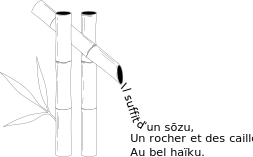
\includegraphics[width=7.5cm]{haiku.pdf}
\end{floatpoem}

\poemtitle{Malin génie}
\begin{verse}
Me demandais-je en me mirant longuement\\
Qui de moi ou de lui est le reflet,\\
Qui de nous deux vit dans la réalité\\
Quand l’autre me répondit \enquote{Ça dépend !}.
\end{verse}

\afterpage{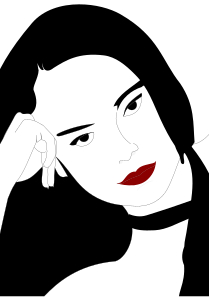
\includepdf[pages={1},addtolist={1,figure,{Mademoiselle F***** au sourcil encoché},encoche}]{portman-encoche.pdf}}
\section*{Trois odes de confinement, autant de quatrains, un zajal, une élégie, une complainte, et un haïku à F*****}
\markboth{}{Trois odes \& quat. zaj. élég. comp. haïk.}
\addcontentsline{toc}{section}{Trois odes de confinement, un zajal, deux quatrains, une élégie, une complainte, et un haïku à F*****}

\begin{prose}
Je rencontrai alors mademoiselle F***** dont la pointe du sourcil gauche est encochée. Il y’a tant de mystères dans l’encoche de ce sourcil que j’en fus intrigué.

Et comme alors je dessinais l’alphabet de Luca di~Borgo aux proportions du nombre d’or, j’entrepris de faire la lettre \autonym{F}, initiale de la demoiselle, en traçant l’attaque de façon encochée.

Je suivi les instruction de di~Borgo, en adaptant les principes président à l’harmonie de ses lettres pour encocher l’attaque de l’\autonym{F}.
\end{prose}




\poemtitle{Tasse renversée}
\begin{verse}
% % Variente en tercet
%Ayant renversé ma tasse sur le tapis,\\
%Je suis  plus déçu pour le contenu exquis :\\
%Le précieux café  que je n’ai pas fini.
%
% Variente en quatrin
Ayant renversée le liquide exquis,\\
Aussitôt affolé je m’en enquis\\
Bien moins soucieux du tapis sali\\
Que du café que je n’ai pas fini.
\end{verse}

\begin{figure}[h]
\centering

\includegraphics[height=2cm]{F.pdf}
\captionsetup{labelformat=empty}
\caption[Lettre \autonym{F} à l’attaque encochée]{}
\end{figure}



\begin{prose}
J’ai souvenir que, pour se rendre à un mariage, elle voulut se faire les sourcils. Je lui suggérai alors de ne les refaire qu’à la condition de conserver cette encoche si singulière.
\end{prose}

\poemtitle[L’exhortation de Ȝumār par le sourcil fendu]{L’exhortation de \fallbackserif{\textbf{Ȝ}}umār\endnote{On rapporte que l’apôtre Ȝumār a annoncé \enquote{Apprenez à vos enfants l’archerie, la natation, et l’équitation}. Or, chaqu’une des trois premières strophes de ce poème s’attache à l’une de ces disciplines en constituant alors un triptyque.} par le sourcil fendu}
\begin{verse}
Le sourcil fendu à la pointe double\\
Qui s’encoche à l’arcade sourcière\\
Bandée par la mydriase si singulière\\
Me prend pour cible et me trouble,

Me projette sur les eaux d’un océan.\\
Par les deux pans qui sont les sillons,\\
D’une brasse haletante mais pélage\endnote{Hapax dû à la licence poétique. De \autonym{pélagique}, \enquote{de haute mer}.}\\
Me fait échoir épuisé sur le rivage

Où une jument fouette de sa queue\\
Qui, dans le vent, se scinde en deux.\\
La chevauchant, Zulfixār\endnote{Épée à pointe double que Mahomet a trouvé dans le butin de la bataille de Badr.} en main,\\
Elle m’entraine jusqu’au lointain.

Mystère de la disgrâce qui se fit victoire.\\
Surlignant de l’encre pileuse l’iris \xenism{barroco}\endnote{Du portugais \xenism{barroco}, désigne en joaillerie une pierre belle parcequ’irrégulière.}\label{foot.barroco},\\
Kintsungi\endnote{Du japonais 金継ぎ \enquote{jointure d’or}, désigne une technique de céramique brisée dont en suite les morceaux sont rassemblés par une jointure d’or, lui conférant un plus bel aspect que si elle était intacte. À rapprocher de la note \ref{foot.barroco}.} rendit-elle le mammaire ivoire\\
Entrainant les vibrations de mes pectoraux.
\end{verse}

%\begin{figure}
%\centering
%\includegraphics[width=0.70\textwidth]{tripaedie.pdf}
%\captionsetup{labelformat=empty}
%\caption[Tripaédie ou éducation par les trois disciplines]{}
%\end{figure}


\poemtitle{Un sourire et j’anhéle}
\begin{verse}
Elle projette les aurores radiales\\
Lorsque, retroussant le bourrelet labial,\\
Les commissures de ses lèvres se renâclent,\\
Poignardant de fougue mon thorax en débâcle.

Ce sentiment haletant,\\
Aspire l’air ambiant,\\
L’engouffre dans les poumons,\\
Et l’expire promptement.

\end{verse}

\poemtitle{La faufilade sous le chemisier}
\begin{verse}
Souple est l’orbe voluptueux,\\
Serti du rubis le plus précieux.\\
Porté en avant, orgueilleux et galbé,\\
Il est de la reine la fierté.

Tenu en main, son verni de velours\\
Submerge de la languissante volupté\\
Et s’en va alors fleurir et enfler\\
Car de tendresse flatté à son tour.

Hallebardier est l’outremer chemisier,\\
Celui aux pépites d’or parsemé,\\
Sous lequel une herse sévère entrave,\\
Avec de l’amante le regard grave.

Sur les tours cylindres\endnotemark[\getrefnumber{foot.tourRonde}], les assauts font défection\\
Mais autour de l’imprenable citadelle sphérique,\\
La belle rotondité accroit l’arduité mégalithique,\\
Dont les attraits obstinent cependant l’assaillant.
\end{verse}


%\paragraph{}
\begin{prose}
Ce poème écrit en maghrebi, le dialecte marocain, langue qui \caution{malgré son apparente ressemblance avec l’arabe littéral du fait de quantité de racines, tiendrait davantage du carthaginois}.

Il aborde dans un style proche du genre musical ca\fallbackserif{ȝ}bi \incise{que j’honni pourtant} des thèmes enracinés dans un tropisme marocain et sans doute même passéiste. Mais dont les préoccupations animent à s’y méprendre les contemporains.

La traduction qui en est donnée, qu’après réflexions je voulu davantage littérale quoique s’accommodant de quelques adaptations plus littéraires, trahis forcément les rîmes et la métrique.
J’avais pourtant fermement songé à rendre le texte maghrébi par un équivalent littéraire qui sacrifierais sans hésiter le sens pour ne conserver que l’exaltation qui en est ressentie. Choix auquel j’ai, sans doute à tort, fini par renoncé.
\end{prose}

\pagebreak
\begin{longtable}{R{0.3\textwidth} L{0.65\textwidth}}
\noalign{\vspace{-0.5cm}\poemtitle[Zajal d’un insomniaque épris — \textarabic{زجل العشّاق الصهران}]{\textarabic{زجل العشّاق الصهران} — Zajal d’un insomniaque épris}}
\endfirsthead

\textarabic{أنا بالليل}                  &       Dans mes nuits,   \\
\textarabic{حاضي الگمرا لا تطير.}         &       Je veille à ce que la lune ne croule.   \\
\\
\textarabic{ضال فايق،}                   &       Demeurant éveillé,   \\
\textarabic{و فبالي صوت الضقايق،}        &       L’esprit des percutions de cuivre imbibé,   \\
\\
\textarabic{راني خايف}                   &       Je crains   \\
\textarabic{لَي جي يقجني السّالف.}         &       Que la longue natte vienne m’étrangler.   \\
\\
\textarabic{و معا الغربي،}               &       Et avec le zéphyr,   \\
\textarabic{يطيّر ما باقى دنعاسي.}        &       Sera ravi ce qui me reste de sommeil.   \\
\\
\textarabic{نفكّر فالغزال}                &       Je songe à la belle   \\
\textarabic{لي گع ميخطى البال.}          &       Qui ne quitte jamais mes pensées.   \\
\\
\textarabic{منفخا عليىا}                 &       Me dédaignant,   \\
\textarabic{و متخصر حتا شوفى فيا.}       &       Elle ne m’accorde pas un seul regard.   \\
\\
\textarabic{ورى الشبيك}                  &       À travers le moucharabieh   \\
\textarabic{ما تورّي لجيهتي غير الشيك}    &       Elle ne me laisse paraitre que la superbe   \\
\\
\textarabic{وخى هكّاك،}                   &       Et malgré tout,   \\
\textarabic{من الشريكة متبوس الحناك.}    &       De la rivale elle ne daigne embrasser les joues.   \\
\\
\textarabic{مولات التاج}                  &       La dépositaire de la couronne,   \\
\textarabic{إلى سمعات غيرها تعواج.}      &       Si elle vient à entendre parler d’une autre qu’elle, se contrarie.   \\
\\
\textarabic{گع النهار،}                  &       Toute la journée,   \\
\textarabic{منها ما نشوف غير الضهر.}     &       Je ne perçois d’elle que le dos.   \\
\\
\textarabic{بكترت ما جميل}               &       Par tant de beauté,   \\
\textarabic{شعرها الكحل غلب الليل}       &       Ses cheveux noirs vainquent la nuit.   \\
\\
\textarabic{طول من النّيل}                &       Plus long que le Nil,   \\
\textarabic{و ضلامو يطفي الپيل.}          &       Son obscurité éteint la lampe-torche.   \\
\\
\textarabic{الگمرا ولات فطحا}             &       La lune parait platte  \\
\textarabic{فحضره گلستها المالحا.}       &       À l’avènement de son assise raffinée.   \\
\\
\textarabic{الزيف \xenism{الريض} (الحمر)}         &       Si le voile \xenism{red} (rouge)   \\
\textarabic{الا مشا حتا زلق نفيض.}        &       Vient à glisser, je fond.   \\
\\
\textarabic{لعندي،}                      &       Vers moi,   \\
\textarabic{راهى حالفا ربي لا تجي.}       &       Elle jure par Dieu de ne jamais venir.   \\
\\
\textarabic{بلا كوڤيد}                    &       Sans covid,   \\
\textarabic{فراقها خلاني مريض.}            &       La séparation me laisse malade. \\
\\
\textarabic{معا ليالي،}                  &       Avec mes nuits,   \\
\textarabic{دّات لي حتى قلبي.}            &       Elle a emporté jusqu’à mon cœur.   \\
\\
\textarabic{تا من العقل}                 &       Et mon encéphale aussi   \\
\textarabic{ولّا كي الآلة فالمعمل.}        &       Est devenu tel l’engin de l’usine.   \\
\\
\textarabic{يضل يخدم}                    &       Il demeure en fonction   \\
\textarabic{ميمشي منو الهمّ.}             &       Et ne se défait de l’anxiété.   \\
\\
\textarabic{شغادي يصنع}                  &       Qu’escompte produire   \\
\textarabic{لي حتا امّ الربيع ميقطع؟}     &       Ce qui ne traverse le fleuve d’Um~al~rabiȝ\endnote{Fleuve usuelement graphié \autonym{Oum Errabiâ} prenant sa source aux environs de Khénifra  et débouchant vers les environs d’Azemmour dans l’océan Atlantique. De ce fait, un voyageur qui irait de Kénitra à Eljadida, le traverserait.}\,?   \\
\\
\textarabic{لي بغي يزيد}                 &       Celui qui s’avance   \\
\textarabic{من مهديه لسيدي بوزيد}        &       De Mehdia vers Sidi~Bouzid\endnote{Communes respectivement proches de Kénitra et d’Eljadida.} \\
\\
\textarabic{يبقى يتجّر}                   &       Demeure entrainé   \\
\textarabic{فاليل حتى يودّن الفجر.}       &       Dans la nuit jusqu’à ce que retentisse  l’aurore\endnote{Le texte marocain utilise le mot \textarabic{فجر} (\xenism{fajr}) soit une allusion à la prière de l’aurore. D’où le retentissement dû à l’\xenism{āḋān}.}.   \\
\\
\textarabic{ربي العالي}                  &       Grand Dieu,   \\
\textarabic{بغيت منها غير الشفاري}       &       Je n’espère d’elle que (voir) les paupières   \\
\\
\textarabic{و إلى ما لقيتها}             &       Et si je ne la trouve pas,   \\
\textarabic{نضلّ نقلّب على القافية.}       &       Je poursuivrais la recherche des rîmes.   \\
\end{longtable}

\poemtitle{La voir dans la nuit}
\begin{verse}
L’ardeur qui me pousse à l’admirer malgré la nuit\\
Contraint ma perception à la nyctalopie,\\
Si bien qu’en son absence tout parait odieux\\
Et y est préférable de se crever les yeux.
\end{verse}

\begin{prose}
Dans un café, J’attendais F***** ou même un signe de sa part, un appel téléphonique, un message. Tandis que le temps passait, des noix de palmiers tombaient à intervalle plus ou moins régulier, comme pour ponctuer le défilement du temps.
\end{prose}

\poemtitle{À distance}
\begin{verse}
Un amour que peut-être nous tisserons\\
Par delà les montagnes et océans\\
Avec l’RJ45 pour fil\\
Mais le chas est trop étroit pour qu’on l’enfile.
\end{verse}

\poemtitle{L’absence}
\begin{verse}
Gorgée après gorgée,\\
Mon verre s’est vidé.\\
Et l’anse ne saurait,\\
À tes bras, suppléer.
%Et l’anse ne saura\\
%tes bras substituer\\

\emph{Ô yeux, ô nuit, ô nuit, ô yeux.}

Ô, voix de plus en plus moindre\\
Qui tombe comme l’averse\\
Ne peut suffire à éteindre\\
Le brasier qui me traverse.

\emph{Ô nuit, ô yeux, ô nuit, ô yeux.}

Maudit instant où, de mon verre,\\
N’apparaît que fin liseré\\
Où subsiste peu de café.\\
J’ignore en vérité qu’en faire.\\
Assurément qu’à l’achever\\
Je me résoudrais que par fer.

\emph{Ô yeux, ô nuit, ô yeux, ô nuit.}

Le palmier qui laisse échoir ses noix,\\
Dont la pourtant sévère  cadence\\
Rappelle ta si pénible absence,\\
À mes cotés pleure mon désarrois.

\emph{Ô nuit, ô nuit, ô yeux, ô yeux.}

Lorsqu’avec grande flagrance, ton rôle\\
Dissone d’avec tes rares paroles\\
Pour quels choix, dis-moi, puis-je encore opter\\
Tandis que tu ne veux t’en expliquer ?

\emph{Ô nuit, ô yeux, ô yeux, ô nuit.}

Concède et pardonne\\
Qu’aux yeux me fixant\\
Gorgés d’océans\\
Je m’ abandonne

\emph{Ô yeux, ô nuit, ô nuit, ô yeux.}

Toi qui ailleurs dirige le mât\\
En fait de tout louvoyant discours,\\
Si tu dubites de mon amour,\\
Regarde ma vulve et tu saura.
\end{verse}

\poemtitle{Du naufrage}
\begin{verse}
J’ai perdu ma proue\\
Et mon navire a coulé,\\
Dans l’eau, tout entier.
\end{verse}

\begin{figure}[h]
\centering
\includegraphics[width=0.9\textwidth]{farir.pdf}
\captionsetup{labelformat=empty}
\caption[Idéotexte du \autonym{vide} (\textarabic{خالي})]{}
\end{figure}

\begin{prose}
Me trouvant non loin du musée de la banque centrale du Maroc, je me dis qu’il valait encore mieux y noyer ma peine. Grand bien me pris car alors \incise{joi} bien loin de m’en douter, j’y trouvais des éléments prélevés sur le site archéologique d’Aghmat, des parties de la maison d’Al\,Mutamid Ibn~Abbad qui commandita à Lissān~al\,Ḋḋīne ibn~al\,Xatīb des poèmes à graver sur ses murs. Mais plus bouleversant encore, un manuscrit que je crus comprendre autographe de Lissān~al\,Ḋḋīne ! Fort heureusement, le masque que je portais du fait de l’épidémie m’épargna le ridicule d’exposer aux gens les larmes qui coulèrent le long de mes joues. Je me suis même retenu de m’assoir par terre tant me jambes s’étaient vidées de leur tonus.

Je dois toute fois être honnête, je n’ai pas pris la peine de vérifier que les manuscrits étaient bien autographes comme j’ai cru le comprendre ; ou plus exactement j’ai soigneusement évité de m’en assurer, préférant me complaire dans l’idée qu’ils l’étaient.
\end{prose}

%\paragraph{}
\poemtitle[Le Zurbiy]{Le \xenism{Zurbiy}\endnote{Le dernier sultan de Grenade, Mohammed XII de Grenade, dit al\,Zurbiy \xenism{l’infortuné} fut le dernier souverain musulman d’al\,Andalous.}}
\begin{verse}
Comme un prince de son royaume banni,\\
Qui ne reverra plus  son Andalousie,\\
De notre amour, l’échec et mat\\
M’est aussi odieux qu’Aghmat.\endnote{Al\,Mutamid Ibn~Abbad  qui a été roi de Séville, fût destitué par les Almoravides pour être exilé à Aghmat où il mourus.}

Que vienne me voir le double-visir\endnote{Allusion à Lissān~al\,Ḋḋīne ibn~al\,Xatīb, savant qui fut par deux fois ministre aux cours nasride et mérinide, ce qui lui valut le surnom de \enquote{celui aux deux visirat} \textarabic{ذي الوزارتين}. Lors de son exil à Aghmat, Al\,Mutamid Ibn~Abbad fit appel à ses services de poète pour rédiger des vers qui furent calligraphiés sur les murs de sa maison.}\\
Et qu’avec ses royaux vers enchanteurs,\\
Ceux qui sont gravés loin sur les hauteurs,\\
Soit marquée l’extinction du désir.
\end{verse}

\section*{Kénitra}
\markboth{}{Kénitra}
\addcontentsline{toc}{section}{Kénitra}

\poemtitle{Matin}
\begin{verse}
Dans la ville engourdie où larmoie le brouillard\\
Fendu par quelques néons à l’éclat criard,\\
Les rideaux encore baissés des magasins\\
Sont aussi lourds que les paupières le matin.
\end{verse}

\poemtitle{L’étudiante}
\begin{verse}
Pour voir les lueurs du jour qui débutait,\\
Je m’étais levé le matin de bonheur\\
Où le premier rayon ayant touché terre\\
Me demanda où était la faculté.\\
Ah, que ne lui aurais-je fais cours sur l’heure\\
Si j’avais eu un grade universitaire.
\end{verse}

\begin{prose}
Je prononçais le quatrain suivant un matin de janvier dans un café où je me retrouvais avec une amie  qui, en se coiffant, s’en révélera être la muse.
\end{prose}

\poemtitle{La crinière}
\begin{verse}
Elle tenait dans sa bouche ses cheveux\\
Tandis qu’elle se peignait la crinière\\
Comme l’on fait tenir le mord aux chevaux\\
Et moi, je la regardais sans œillères.
\end{verse}

\begin{prose}
Si heureux de l’avoir composé, j’ouvris mon journal et tout le monde me vit esquisser un large sourire de satisfaction en lisant un article intitulé \work{Armes françaises pour dictature exemplaire}.
\end{prose}

\poemtitle{Du soleil dans mon café}
\begin{verse}
Instant sans pareil\\
Que celui où le soleil\\
Pointe son premier rayon\\
Sur mon guéridon.
\end{verse}

\poemtitle{Le vert talus}
\begin{verse}
Accompagnes-moi au vert talus.\\
Je t’en prie, viens t’y prélasser.\\
Tu y trouvera le salut\\
Dans lequel tu pourra rêvasser.
\end{verse}

\poemtitle{Le regard bleu}
\begin{verse}
Devant son regard bleu où s’ouvre un détroit\\
Celui qui en séparant deux continents,\\
Éloigne les nefs achéennes de Troie\\
Comment n’éprouverais-je aucun sentiment ?
\end{verse}

\poemtitle{Collision}
\begin{verse}
Flottant dans la flaque d’eau violette,\\
Les jets de lumière des lampadaires\\
Vinrent s’éclabousser sur mes lunettes\\
Quand t’arrive dessus en roue arrière.

Tu es passée à moto devant moi,\\
Et si tu as failli me renverser\\
J’ai tout de même scandé un verset\\
Car je suis mort quand tu me regardas.
\end{verse}

\poemtitle{Réminiscence de l’infante du Portugal}
\begin{verse}
Ces yeux de saudade\\
Où se déploient les Cyclades\\
Me font une œillade.
\end{verse}

\begin{figure}[h]
\centering
\includegraphics[width=\textwidth]{img/ines-syntwave.pdf}
\captionsetup{labelformat=empty}
\caption[Portrait syntwave d’Inèss]{}
\end{figure}

\begin{prose}
Je passais avec Inèss une de ces journées dont on parlera encore dans les siècles des siècles. Ne vous ai-je jamais parlé d’elle ? Nul besoin, l’ensemble de l’ouvrage est teinté de son emprunte.

C’était une journée de juillet, c’en était la dernière. Je la passais avec la ravisante Inès. Et c’était comme un verre de caffé vide que l’on penche éspérant ne rien gaspiller des ultimes goutes qu’il peut peut-être encore contenir, ou s’il n’en réste pas, se faire croire que l’on a pu tout de même en grapiller.
Quelle ne fut pas notre surprise, lorsque le mois de juillet s’avéra magicien car son verre avait un fond caché !

D’autan que, et vous pourrez immaginer à quel point nous étions enjoués, Inès venait tout juste d’acquérir une automobile pour la première fois. C’était un prélude au mois d’aôut.

Nous étions au 2021 juillet 31 et, tandis que fendaient sur nous les rayons crépusculaires, nous prenions la route, lunettes de soleil au museau en écoutant de la syntwave.
\end{prose}

\poemtitle{Virée d’avant août}
\begin{verse}
Toi et moi, sur l’écran de cinéma,\\
Nous roulons droit devant vers l’horizon,\\
Vers tous nos rêves et nos passions\\
Loin de la sombreur du pont de l’Alma.

Je veux capturer comme un photographe\\
L’instant précis où tu secoue ta coiffe\\
Qui éclabousse des mèches rebelles,\\
Les reflets des lunettes de soleil.
\end{verse}

\begin{prose}
Le lendemain, toujours en voiture évidement, nous partîmes nous baigner à l’embouchure du fleuve Sebou. Nous grimpâmes  sur les rochers de l’une de ses deux immenses jetées, enjambant les creux, cherchant les chemins les moins éscarpés, pour finalement parvenir à un récif. Après nous être baignés, nous immergeâmes d’entre les vagues et les roches pour aller nous assoir sur un écueil à fleur d’eau. Et tandis que le ressac des vagues sur le rocher qui se faisait plus violent sonait comme une carésse, Inès me demanda \enquote{Y’a-t-il plus heureux que nous dans le monde à cet instant ?}. Qu’avais-je besoin de  répondre lorsque les vagues éteintes trouvaient encore le prolongement de leur beauté autant que de notre enchantement dans l’écume ?

%Là, nous nous baignâmes parmi les roches à fleur d’eau et les écueils.
\end{prose}

\poemtitle{Baignade avec Inès}
\begin{verse}
Caressée par les vaguelettes turquoise,\\
Est-ce l’eau qui la baigneuse a embellie\\
Ou est-ce sa beauté qui y déteignit,\\
Tant la mer devint diamant et topaze ?

Je compris pourquoi la mer est si belle.\\
Souvenez-vous qu’au contact de sa peau,\\
L’éclat d’Inès y laissa des séquelles,\\
À chaque fois que vous boirez de son eau.
\end{verse}

\begin{prose}
J’étais à Kénitra où j’allais me faire injecter ma première dose de vaccin. En chemin, je regardais une jeunne femme qui m’inspirait. Et déjà j’immaginais mes amis à qui je racontrait la scène qui me railleraient, me demandant si toutes m’inspiraient. Commençant à composer une réponse à cette question immaginaire, je me me disais \enquote{Ne mérite-t-elle pas un poème}.

Je réféléchis alors à une  suite sans me douter qu’elle viendrait d’elle même lorsque je me serais rendu compte de ne pas être le seul à observer cette passante.
\end{prose}

%\poemtitle{Le sermon}
%\begin{verse}
%Nous prêtâmes sermon\\
%Sous les hiéroglyphes\\
%En est témoin le sang\\
%Apposé de nos griffes.
%\end{verse}

\poemtitle{La muse}
\begin{verse}
Ne mérite-t-elle pas un poème ?\\
\enquote{Si, bien sûr que si !} clamait le cycliste\\
Quand, la regardant le visage blême,\\
Le fourgon le renversa sur la piste.
\end{verse}


\poemtitle{Le bien inspiré}
\begin{verse}
L’on dit que j’écris au sujet des femmes,\\
Mais rien n’est plus faux, je ne suis que l’arme,\\
Quand elles me trempent dans la cyprine\\
Et me font transcrire l’humeur chagrine.
\end{verse}

\poemtitle{Torche}
\begin{verse}
Les flammes de cheveux voltigeant au vent proche\\
Ce n’était pas une femme mais une torche.\\
Si sa taille semble se caler dans la main\\
Je la saisirais pour éclairer mon chemin.
\end{verse}

\poemtitle{Déception}
\begin{verse}
Quelque chose en moi se brisa\\
Pourtant, rien n’eu lieux ce jour là.\\
Certes, pas grand chose en tout cas,\\
Quoique ce fut beaucoup pour moi.

Un détail, un foutu détail.\\
De ceux qui sont déterminants,\\
De ceux sonnent comme une faille,\\
Qui s’annoncent fatalement.
\end{verse}

\poemtitle{Réminiscence de l’infante du Portugal}
\begin{verse}
Ces yeux de saudade\\
Où se déploient les Cyclades\\
Me font une œillade.
\end{verse}

\poemtitle{Cosmopolite}
\begin{verse}
J’ai arpenté Doura-Europos\\
Et ai sillonné ses avenues.\\
C’est alors ma cité que j’ai vu\\
Car je suis citoyen du cosmos.
\end{verse}

\poemtitle{Collère}
\begin{verse}
Pour les dérober aux maints regards,\\
Il enfouit ses ressentiments\\
Ici, sous des profondeurs souterraines\\
Si vastes que de leur déblaiement\\
Émergea un tertre trop voyant,\\
Qui inscrivit les traits de la haine\\
Sur son visage blême et hagard.
\end{verse}



\poemtitle{Le surfléché}
\begin{verse}
Comme un soldat tombé au sol car sur-fléché\\
Qui scrute le champs d’honneur avant d’abdiquer\\
Et sur lequel pleuvent les flèches acérées,\\
Je suis assailli de ses  baisers enflammés.
\end{verse}

\poemtitle[Le nay]{Le nay\endnote{Flûte à l’origine perse d’où elle tire son nom signifiant \autonym{roseau}, mais aussi turque et arabe intervenant en général dans le répertoire de la musique savante.}}
\begin{verse}
Que le musicien prenne son nay,\\
Qu’il en insuffle l’air sacré dans nos âmes,\\
L’air qui apaise et fait déposer les armes\\
Et qu’avec, les turpitudes s’en aillent.
\end{verse}

\poemtitle{Sac de la bibliothèque d’Alexandrie}
\begin{verse}
Tel l’aveugle qui me toise en étant ivre\\
Et me regarde alors de ses globes vides,\\
La bibliothèque dégarnies de livres\\
Est un paysage insipide et livide.
\end{verse}

\poemtitle{Appelle-moi}
\begin{verse}
Khadija, appelle-moi ce soir\\
Et nous braverons le couvre-feu\\
Dans la nuit qui dérobe aux regards\\
L’ardeur de nos jeux facétieux.

Les rideaux tombent, il est neuf heure.\\
Angle Mohamed~\textsc{v}—Diouri,\\
Viens y en ramenant des souchis\\
Et j’apporterais ma bonne humeur.

Khadija, viens me voir en voiture,\\
Et nous prendrons d’asseau Kénitra\\
Qui pour nous sera des rues de Troie\\
Où nous deux courrons vers l’aventure.

Khadija, appelle moi ce soir\\
Et le  café tombe de mes mains.\\
À tout le reste je vais surseoir,\\
Livré à tes bras jusqu’à demain.

Khadija, appelle moi ce soir\\
Et se lèvera une traînée\\
Dans mon dos, quand j’ai filé te voir\\
Quelques chats en furent effrayés.

Khadija, appelle moi ce soir.\\
Crois-moi, Starship me jalousera\\
Car j’atterrirais où que tu sois\\
Mieux que Mars ce sera pour te voir.
\end{verse}

% la femme écrite
\begin{prose}
Fût donné à Kénitra une projection de \work{La Femme écrite} à laquelle était présent le réalisateur Lahcen \textsc{Zinoun} pour une séance d’entretiens. Ce film me démangeait. Il m’a semblé qu’une parade nuptiale berbère prenait les accents de l’habanera \work{Carmen} de \textsc{Bizet}. À un autre moment, j’ai cru voir une allusion à \work{Body Double} de Brian \textsc{De Palma}, quand certains plans ne me faisaient pas carrément penser à la série des odalisques d’\textsc{Ingres} tant elles semblaient en être décalquées. J’avais tant de questions dis-je, et si peu de temps, et en même temps, la description qui y était faite de la sexualité et de la sensualité me semblait parenter avec de la stratégie militaire. Comme si un nouveau milieu stratégique s’était ouvert. Je retins particulièrement que dans son film, les femmes sur la peau desquelles s’inscrivent des textes avant d’être brisées me semblèrent être des ostracons, et quelle ne fût pas ma surprise lorsque par la suite le réalisateur prit la parole pour les qualifier de palimpsestes.

\begin{figure}[h]
\centering
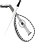
\includegraphics[width=0.33\textwidth]{sautoir-doud-et-dépée-monochrome.pdf}
\captionsetup{labelformat=empty}
\caption[Oud et épée ulfberht passés en sautoir]{}
\end{figure}

Ce film me démangeait, j’avais tant de choses à demander à son réalisateur alors présent, si bien qu’une idée chassant l’autre, je ne pu poser toutes mes questions. Finalement, j’ai pu demander à M.\,Lahcen \textsc{Zinoun} si la ressemblance entre certaines scènes et les odalisques d’\textsc{Ingres} n’étaient qu’un effet de ma sur-interprétation ou bien une référence voulue. Si je vous demandais de deviner ce qu’il me dit, c’est que dans ma question réside déjà la réponse; eh bien il me confirma son intention de faire allusion aux toiles d’\textsc{Ingres}.

Mais devinez d’abord qui m’accompagna ce jour là à la projection de ce film. Sauf qu’évidement, je ne peux vous poser cette énigme sans que vous ne vous doutassiez déjà de la réponse car évidement que j’étais avec Inès.
\end{prose}

\poemtitle{Premier milieu stratégique}
\begin{verse}
Ter, mer, ciel, espace, et jusqu’au cyber-espace\\
Tels sont les cinq milieux que l’on enseigne aux classes\\
Mais le plus ancien de ceux que connaît la guerre\\
Dans les écoles d’armée ne s’enseigne guère.

Car si la guerre est un récit\\
Qui s’écrit sur les corps aussi\\
Ceux des femmes sont palimpsestes des amants\\
Mais meurtri des conflits, ils ne sont qu’ostracon.

Un champs certes sont les corps des femmes\\
Est-ce de bataille ou de labour ?\\
Rien n’est moins sûr dans cet amalgame\\
Où la guerre se mêle à l’amour.
\end{verse}



\poemtitle{Nakano Takeko}
\begin{verse}
Nakano, tel le feu,\\
Sous cloche, elle s’éteint\\
Mais libre elle s’étend,\\
Dans un élan fougueux\\
Fait de cuivre et d’éteint\\
Jusqu’à l’ignition.
\end{verse}

\poemtitle{Poliorcète}
\begin{verse}
Par son regard de braise si ardent\\
Qui consuma mon cœur lors de la défaite,\\
Je prends d’asseau le sien en poliorcète,\\
Autant assiégé qu’assiégeant.
\end{verse}

\poemtitle{Café turque}
\begin{verse}
Constantinople prise par l’ivoire,\\
Même mille fois, ne saurait valoir\\
Ô Turques, votre plus grande victoire,\\
Celle du café que je m’en vais boire.

Contre les croisés, peu me chaud\\
L’issue de toutes vos batailles\\
Car avec le breuvage chaud\\
Il n’est de querelle qui vaille.

Les épices, comme autant d’odalisques,\\
Valent toutes les femmes du sérail.\\
La brune au goût de musc à peine bisque\\
Ou la rousse de cannelle m’assaillent.

Que d’autres Talas\endnote{Bataille de la rivière Talas ayant opposé le califat abbasside à la dynastie Tang pour le contrôle de la Transoxiane et au cours de laquelle les mercenaires turques Karlouks alliés des Chinois font volte-face au profit des abassides ancrant depuis lors les peuple turques dans le monde musulman.} aient encore lieux,\\
\incise{Cent Talas} pour qu’autan de fois encore\\
Soit notre ce café délicieux,\\
Et le papier\endnote{Il est probable que les captifs Chinois fait par les Abbassides au cours de la bataille de Talas aient introduit dans le monde musulman les techniques de fabrication du papier, donnant par conséquent le coup d’envoit à l’âge d’or arabomusulman.} où j’écris ces mots d’or.
\end{verse}

\poemtitle{La cours des Lions}
\begin{verse}
On s’assit aux bords d’une fontaine\\
Dont les flots, de nuit, nous arrosaient\\
Abreuvant nos paroles mondaines\\
Où fût conviée la roseraie.

Ayant palabré de tant de choses\\
Jusqu’aux primes lueurs de l’aurore\\
Où nous devinrent bouton de rose,\\
Je ne su si nous pouvions éclore.
\end{verse}

\poemtitle{L’Antisocrate}
\begin{verse}
Ses paroles, je les bues comme la ciguë\\
Mais ce fut moins pour avoir eu de la sagesse\\
Que pour en avoir alors été dépourvu,\\
Tant elles m’enivrèrent de leste allégresse.
\end{verse}


\poemtitle{Signum minimum}
\begin{verse}
On dormit dans la nuit de Talassemtane\\
Entre les montagnes et les bêtes fauve\\
Avec la voûte céleste pour alcôve\\
Dont s’accommoda avec joie ma sultane.

L’enlaçant de mes ailes de grand-duc,\\
Mon souffle chaud lui caressant la nuque,\\
Je lui susurrait à l’oreille en chuintant :\\
\enquote{Y’a-t-il plus heureux que nous en cet instant ?}

Mais qu’avait-elle besoin de répondre, elle,\\
Quand les fières étoiles peuplant le ciel\\
Qui flottent solitaires aux alizés,\\
Lasses de nous admirer, nous jalousaient ?
\end{verse}

%\begin{verse}
%\end{verse}
%\begin{adjustwidth}{-2.5cm}{0cm}%

\begin{prose}
Je suis tombé devant une copie du \work{Massacre des Abencérages} de Mariano \textsc{Fortuny} qui me saisit d’effroi, non pas tant pour le sujet sinistre et lugubre représenté, que par la violence par laquelle j’y fût projeté. Je m’actualisais immédiatement dans ce tableau où comme par réalité augmenté, je me suis retrouvé. J’aurais pu me mouvoir au sein de cette cours des Lions, sentir sur la plante de mes pieds le sang frais du gisant où j’ai marché, tant je me suis senti familier du propos.

Aussi ai-je ressenti… ou plutôt ai-je été saisi par l’effroi du thème abordé, celui de la dramatique chute des Abencérages qui n’est qu’un prélude à celui du royaume de Grenade et enfin d’Al-Andalous. Et spontanément, les vers s’imposèrent à moi en latin.
\end{prose}
\poemtitle{\xenism{Abenceragi} — Abencérages}
\setlength\LTleft{-1.7cm}%
\begin{verse}
Abenceragi, vos Elviræ domini,           \\
Sanguis vester Alhambræ fontem adaquat,  \\
Quæ suum nomen numquam tam bene gerebat. \\
Non potentes estis sed adberitani.       

\emph{Abencérages\endnote{Famille puissante d’Al-Andalous.}, vous maitres de Grenade,}\\
\emph{Votre sang abreuve les fontaines de l’Alhambra,\endnote{Allusion à la légende de leur éxtermination dans un bain de sang dont on raporte : \enquote{La fontaine d’apparat ne laissait plus couler de l’eau, mais leur sang…}.}}\\
\emph{Qui jamais ne portât aussi bien son nom.\endnote{\autonym{Alhambra} de l’arabe \textarabic{الحمراء}, voulant dire \autonym{La Rouge}.}}\\
\emph{Vous n’êtes pas puissants mais adbéritains\endnote{À comprendre dans le sens que la poésie latine lui donne de \emph{sôt}, \emph{stupide}.}.}

Damno vestram nefas rixam cum Ziridis   \\
Quam totum Gratæ regnum tecum perdidit. \\
Si pater vester sutor fortasse fuierit, \\
Infra antecessorum soleam nunc estis.   

\emph{Maudite soit votre querelle avec les Zirides\endnote{Faction rivale des Abencérages dont le conflit ensanglanta Grenade au point d’en hâter la chute.}}\\
\emph{Où vous entrainâtes dans la destruction le royaume de Grenade}\\
\emph{Si votre père fut sans doute cordonnier\endnote{\autonym{Abencérage} de l’arabe \textarabic{بنو سراج}, voulant dire \enquote{fils de cordonier}.},}\\
\emph{Vous êtes sous les sandales de vos ancêtres désormais.}
\end{verse}

%\begin{longtable}{L{7.3cm} L{6.5cm}}
%\noalign{\poemtitle{Abencérages — \xenism{Abenceragi}}}
%\endfirsthead
%
%Abenceragi, vos Elviræ domini, & \emph{Abencérages\endnote{Famille puissante d’Al-Andalous.}, vous maitres de Grenade,}\\
%Sanguis vester Alhambræ fontem adaquat, & \emph{Votre sang abreuve les fontaines de l’Alhambra,\endnote{Allusion à la légende de leur éxtermination dans un bain de sang dont on raporte : \enquote{La fontaine d’apparat ne laissait plus couler de l’eau, mais leur sang…}.}}\\
%Quæ suum nomen numquam tam bene gerebat. & \emph{Qui jamais ne portât aussi bien son nom.\endnote{\autonym{Alhambra} de l’arabe \textarabic{الحمراء}, voulant dire \autonym{La Rouge}.}}\\
%Non potentes estis sed adberitani. & \emph{Vous n’êtes pas puissants mais adbéritains\endnote{À comprendre dans le sens que la poésie latine lui donne de \emph{sôt}, \emph{stupide}.}.}\\
%\\
%Damno vestram nefas rixam cum Ziridis & \emph{Maudite soit votre querelle avec les Zirides\endnote{Faction rivale des Abencérages dont le conflit ensanglanta Grenade au point d’en hâter la chute.}}\\
%Quam totum Gratæ regnum tecum perdidit. & \emph{Où vous entrainâtes dans la destruction le royaume de Grenade}\\
%Si pater vester sutor fortasse fuierit, & \emph{Si votre père fut peut-être cordonnier\endnote{\autonym{Abencerage} de l’arabe \textarabic{بنو سراج}, voulant dire \enquote{fils de cordonier}.},}\\
%Infra antecessorum soleam nunc estis. & \emph{Vous êtes sous les sandales de vos ancêtres désormais.}
%\end{longtable}
%%\end{adjustwidth}

\poemtitle{Aube}
\begin{verse}
Les rayons du soleil comme autant de pinceaux\\
Peignent  la nuit lorsque s’en appose le sceau\\
En y parsemant la couleur chaire des femmes\\
Mais qui, à l’arrivée de l’aurore, se fane.
\end{verse}

\poemtitle{Éxhortation au troubadour}
\begin{verse}
Ô troubadour, par des airs attrayants,\\
Captives-nous et déploie ton talent.
\end{verse}

\poemtitle{La Nébuleuse}
\begin{verse}
Elle qui fut mon horizon et mon ciel,\\
Lorsqu’elle rougit à mes propos de miel,\\
C’est d’un crépuscule écarlate céleste\\
Dont se part son visage et ses gestes lestes.
\end{verse}

\poemtitle{Les enfants du soleil}
\begin{verse}
Nous sommes les enfants du soleil.\\
À nous l’amour à chaque réveil\\
Car, égaux, nous sommes tous pareils,\\
Chacun de nous est une merveille.

Et s’allume dans nos yeux vermeil\\
La passion qui se délaye\\
Quand par les rayons l’on se fraye\\
Tous les chemins exceptionnels.
\end{verse}

\poemtitle{Le silence était d’elle}
\begin{verse}
Elle se tait. Dois-je m’exprimer ou me taire ?\\
Commenter la perfection la gâterait,\\
Mais, dans le cas contraire, ne guère parler\\
Laisserait croire qu’elle puisse me déplaire.
\end{verse}

\begin{prose} 
Ne pouvant me résoudre à ne guère aborder de nouveau le cycle \work{Dune}, il me fallut, presque par la force de la nécessité en écrire encore quelques vers, comme autant de précieuses lampées d’eau que l’on craint de verser sur le sable. Et alors que l’excellentissime M.\,Hans \textsc{Zimmer} fut à l’œuvre dans la musique de l’adaptation cinématographique qui en fût faite récemment, c’est en vérité son travail sur le non moins mémorable \work{Interstellaire} qui accompagna \incise{non, que dis-je ?} qui enjoignît mon écriture.
\end{prose}

\poemtitle{Amour sur Arrakis\endnotemark[\getrefnumber{foot.DuneArrakis}]}
\begin{verse}
Dans l’ivresse de l’orgie tau\endnote{Dans l’œuvre de Frank \textsc{Herbert} il s’agit d’orgies sacrées et ritualisées du peuple Fremen.},\\
Je l’ai aimée à en perdre la peau,\\
Jusqu’à en être décharné\\
Comme emporté par la Coriolis\endnote{Type de tempête mortelle dans l’univers de \work{Dune}.},\\
Autant étreins par sa peau lisse,\\
Qu’enlacé de ses deux bras acharné.

Me mirant dans son regard bleu,\\
Le regard de l’ibad\endnotemark[\getrefnumber{foot.regardibad}], serti d’ardeur\\
Me dit combien elle me veut,\\
Qu’elle me désir à pleine fureur\\
En combattante du jihad\\
Qui lutte sur Dune pour notre dyade.

Ô sayyadina\endnote{Sorte de prétresse des Fremen qui guide l’orgie tau.}, hâtes-toi\\
Et transmutes l’eau-de-vie du faiseur\endnote{Le faiseur est une créature sécrétant une eau toxique tant que la sayyadina n’y pratique pas un rituel qui la rend potable.}\\
Afin que le sietch\endnote{Sorte de communauté villageoise de Fremen vivant dans le désert.} en boit\\
Afin que la fremen m’aime sur l’heure\\
Et que dans les couloirs du temps,\\
Avec euphorie nous y entrions.

Ma belle et puissante Fremen,\\
L’âme affûtée par le vent du desert,\\
À la peau de sable et d’ébène,\\
Que l’existence parait si légère\\
Lorsque je demeure sans voix\endnote{Double sens avec la \autonym{Voix} qui est une capacité qu’acquièrent certaines personnes exceptionnelles.},\\
Lorsque ton regard se pose sur moi.

Dégrafant si tôt le distyle\endnote{Vêtement des Fremen qui leur permet de survivre aux rigueurs du désert.}\\
Et négligeant sur le sol la jolitre\endnote{Gourde utilisée par les Fremen pour garder l’eau dans le désert.}\\
Pour se donner au jeu subtile\\
Que l’on reportera sur tant d’épîtres\\
En or et en hiéroglyphes\\
Et dont se souviendront les apocryphes.

Tressaille, fille d’Arrakis.\\
Oh oui, tressaille de cette allégresse\\
Dont t’aura enivrée l’épice.\\
Que soit portés haut tes cris de liesse,\\
Qu’ils se oient bien au delà de Dune\\
Et s’entendent plus loin que ses deux lunes.\endnote{Autour de la planète Arrakis orbitent effectivement deux lunes.}
\end{verse}

\poemtitle{Halène}
\begin{verse}
Et son halène chaude qui me caresse\\
Me fait déjà une secrète promesse,\\
Avant que ses lèvres tendres me sertissent\\
Invitant à un langoureux interstice.
\end{verse}

\poemtitle{Rien de plus}
\begin{verse}
Et tout ce que contiennent le ciel et la terre\\
Ne saurait comme ton sourire te parfaire.
\end{verse}

\poemtitle{Danse de feu}
\begin{verse}
De la lave qu’à travers mes yeux l’on versa,\\
Que cette danse qui consume mon cœur\\
D’un corps liquide qui fait suinter ma sueur.\\
En un instant, elle nous bouleversa.
\end{verse}

\poemtitle{Ordre de bataille}
\begin{verse}
Les arcs, les arbalètes, et les frondes\\
Font pleuvoir une nuée qui abonde\\
De flèches, de vifs carreaux, et de pierres\\
Qui choient autant que tombent les paupières.
\end{verse}


\section*{Didaxie}
\markboth{}{Didaxie}
\addcontentsline{toc}{section}{Didaxie}

\poemtitle{La vie, ses peines, et ses dilemmes}
\begin{verse}
\enquote{Face à la vie et à ses dilemmes,\\
Il n’existe rien de plus à même\\
De panser chacun des maux qui lèsent\\
Que le \work{concerto d’Aranjuez.}}

Nous dit le poète. Mais alors moi,\\
Je crois que c’est plutôt le chocolat !
\end{verse}

\begin{prose}
D’amblais, il me sembla voir une proximité phonétique entre les mots latin d’\autonym{enfant}, \autonym{livre}, et \autonym{liberté}. Serait-ce sans doute parceque les livres libèrent les enfants ? Ce qui se dit :
\end{prose}

\addcontentsline{toc}{subsection}{Maxime de la libération par les livres}
\subparagraph{}
Libri libros liberant.

\poemtitle{Du tenis de table}
\begin{verse}
J’entends ping et pong,\\
Et je tapes, paf, la balle\\
Qui rebond et tombe.
\end{verse}

\begin{figure}[h]
\centering
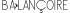
\includegraphics[height=1cm]{balancoire.pdf}
\captionsetup{labelformat=empty}
\caption[Idéotexte de \autonym{balançoire}]{}
\end{figure}

\begin{prose}
Il y’avait, je ne me souviens plus quand exactement, un enfant à qui je devais, pour lui donner un cours de langue, lui illustrer que notre langue n’est pas à la vérité des plus aisée. Je lui donnais l’exemple des mots du cheval et la grande variété des racines pour les former.
\end{prose}


\poemtitle{Les mots du cheval}
\begin{verse}
Prenons un animal,\\
au hasard, le \autonym{cheval}.

Sa femelle, la \autonym{jument}\\
Est une douce maman.

Elle fait des câlins\\
À son petit \autonym{poulain}.

Si jamais on le fait \autonym{hongre},\\
il deviendra castré, bigre !

S’il en est autrement,\\
Il sera \autonym{étalon}.

Luttant avec fierté,\\
Il sera le \autonym{destrier}

Ou distant de l’effroi\\
En charmant \autonym{palefroi}.

Scellé par un \autonym{écuyer},\\
Il mène le \autonym{cavalier}.

Ou au jeu de la paix,\\
Par le beau \autonym{jokey}

Dans une course \autonym{hippique}\\
Qui sera aussi épique

Que nous croyons souvent\\
Être \autonym{équitation}.

Ferres-toi auparavant\\
Par le \autonym{maréchal-ferrant}.
\end{verse}



\section*{Courtes épopées d’arc et de dague}
\markboth{}{Courtes épopées d’arc et de dague}
\addcontentsline{toc}{section}{Courtes épopées d’arc et de dague}
\poemtitle{Exorde à l’archer}
\begin{verse}
Tapisse toi derrière le merlon et encoche\\
La flèche perçant le catafractaire en approche.\\
Tiens-toi devant le créneau et libère\\
La flèche traçant la cuirasse fière.

Dégaine l’épée à la lame damascène,\\
Suspends-en promptement de l’assaillant l’allène.\\
Et le sang qui ruissellera sur le moiré,\\
Séché, sera donc legs à la postérité.

Les faisceaux indéfectibles, par la guivre,\\
Seront noués de sa dépouille languide.\\
Exorde aux justes de s’y rallier\\
Et rappel de l’engeance terrassée.
\end{verse}

\poemtitle{Les dagues des meurtrières}
\begin{verse}
Les cheveux bouclés qui flottent au vent\\
Sont la bannière de celles aux charmes ondulants.\\
Coiffées d’autant de dagues meurtrières,\\
Donnant l’ennemi aux sinuosités de la guerre.
\end{verse}

\poemtitle{Le sang ennemi}
\begin{verse}
Que toujours dans nos coupes, vermeils se déversent\\
Les torrent affluents des  régiments occis.\\
Que toujours dans nos coupes, le sang ennemi\\
Pleuve jusqu’au buvant et remplisse en averses.
\end{verse}



\section*{Constellation du Loup}
\markboth{}{Constellation du Loup}
\addcontentsline{toc}{section}{Constellation du Loup}
\poemtitle{α Lupi}
\begin{verse}
Tant de choses renferme le vaste espace\\
Mais hélas bien peu me chaud ce qui s’y passe.\\
D’entre Balance, Scorpion, ou Centaure,\endnote{La constellation du Loup se trouve entre celles des Balance, Scorpion, et Centaure.}\\
Seule la plus brillante étoile j’explore.

Les longs cheveux noirs de la Beta Cephei\endnote{Les étoiles variables de type Beta Cephei, ou par métonymie les Beta Cephei constituent une catégorie d’étoiles dont fait parti l’alpha Lupi.}\\
Sont des cordes de violon attendries.\\
Délaissant l’archer pour un pizzicato\endnote{Technique de violon consistant à pincer les cordes des doigts au lieux d’utiliser l’archer.},\\
S’y glissent les doigts qui jouent l’adagio\endnote{Deuxième mouvement du \work{Concerto d’Aranjuez} composé par Joaquín \textsc{Rodrigo}.}.

S’effilent de ses rayons des notes si charmantes\\
Que l’on veut toujours longues et éclatantes.\\
Qu’elles ne s’éteignent pas ces quelques braises,\\
Ces notes du \xenism{Concerto de Aranjuez}.

Les savourant de grande admiration,\\
Je perçois de l’or et tant de diamants\\
Dans la voix qui perce le cosmos entier.\\
Il n’est désormais plus Férmi\endnote{Jeu de mot avec le paradoxe de Fermi. Du nom du prix Nobel de physique qui postula une série d’observation et émis des hypothèses au sujet de l’existence de civilisations extraterrestres.} d’en douter.

Perclus de doutes devant le télescope,\\
Au souvenir de la cartomancienne\\
Qui d’Ézéchiel\endnote{Allusion à la carte du Monde dans le tarot de Marseille laquelle arbore le thème du tétramorphe tel que décrits dans la vision d’Ézéchiel.} tira une antienne,\\
Je vis mes tripes dans les vases canope.

Mugissant, glatissant, rugissant, priant\endnote{Chaque cris représente l’un des \enquote{quatre vivants}. Le taureau pour le mugissement, l’aigle pour le glatissement, le lion pour le rugissement, et l’ange pour la prière.}\\
L’arcane émeut l’âme en se l’appropriant.\\
Le Monde qui mit le monde sous des lois,\\
Que gueux et rois admirent de bon aloi.
\end{verse}

\poemtitle{Les feux de tes yeux}
\begin{verse}
Dans l’ardeur calcifère de tes yeux,\\
Se déchaîne ici-bas un ardent feu.

Incendie dont tout l’apostolat\\
Étend loin ses flammes et ses bras.

Au delà de l’Himalaya\\
Et encore bien au delà,

Déclenche l’ignition\\
Qui est la séduction.

Pares-moi de tes ailes,\\
Que j’atteigne le ciel.

Comme ta pupille,\\
La terre scintille

Dans l’atmosphère\\
Où  prolifèrent

Tous les feux\\
De tes yeux.

Les feux\\
Des yeux,

De\\
Tes\\
Yeux.
\end{verse}

\begin{prose}
C’est en sa compagnie à elle, Alpha du Loup, que s’affermit mon gout pour la synthwave qui s’était auparavant manifesté. Tant de choses ai-je appris d’elle, au risque de paraphraser les poèmes où j’en parles déjà.
Et je devrais, pour rendre grâce à l’influence \incise{au rayonnement, allais-je dire} qu’elle eu sur moi en dire beaucoup plus que ces quelques poèmes, mais je trouvais qu’il y’avait, là concernant, grande élégance dans la brièveté.
\end{prose}

\begin{prose}
Du reste, combien même sais-je l’image de la \enquote{bande sonore d’une existence} est éculée, qu’il y’a un lieu commun que je suis le premier à abhorrer, mais le morceau \work{Plastic love} et d’autres encore, plus que jamais m’évoquent la période où je la rencontrai.
\end{prose}

\poemtitle{Maria \textsc{Takeuchi}}
\begin{verse}
Dans mon rêve mauve\\
Elle, Maria \textsc{Takeuchi}\endnote{Allusion à la chanteuse de city pop Maria \textsc{Takeuchi} et à sa chanson プラスチック・ラブ sortie en 1984 connue sous le nom international de \work{Plastic love}, et plus exactement à la résurgence de l’intérêt dont elle fit preuve en 2017 à la faveur d’un algorithme de recommandation et de la popularité des genres esthétiques vaporwave et synthwave qui accompagnent cette période. Autrement dit, cette chanson n’aura connu de succès que trente-trois ans après sa publication. Le regain de popularité pour ce morceau ayant donné lieux à de nombreuses reprises, il me semble qu’est fait ici allusion aussi bien à l’œuvre originale qu’à ses dérivées,  notamment \work{Plastic Love (cyberpunk/synthwave remix)} par Astrophysics publiée en 2020 mars 31.},\\
Chantait en syntwave.
\end{verse}

\begin{figure}[h]
\centering
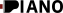
\includegraphics[height=1cm]{piano.pdf}
\captionsetup{labelformat=empty}
\caption[Idéotexte de \autonym{balançoire}]{}
\end{figure}

\begin{prose}
Je ne devrais plus rien ajouter d’autre la concernant, à elle qui composa pour moi de jolies chansons sur son piano, et qui aurait encore probablement fait des symphonies si je n’avais pas fais le con. Mais autant qu’un ivrogne qui prendrait un dernier verre pour la route, je prendrais moi aussi un dernier vers.
\end{prose}

\poemtitle{Aflixion}
\begin{verse}
Aussi tuméfié que moi par le miroir,\\
Ô Quetzalcóatl, laisse tomber quelques plumes\\
%De grâce, laisse en plusieurs encore choir\\
%Qu’il y en ai assez pour le mal qui m’allume,\\
Que je m’en saisisse et écrive mes déboires,\\
Que je puisse en transcrire toute l’amertume.
\end{verse}

\section*{Vers d’autres horizons}%
\markboth{}{Vers d’autres horizons}%
\addcontentsline{toc}{section}{Vers d’autres horizons}%

\poemtitle{Laurier éclatant}
\begin{verse}
Le laurier qui explose en mille émotions,\\
Lance ses fleures en toutes directions,\\
Sous lesquelles les rayons du soleil s’infiltrent,\\
Et de l’astre lumineux apportent l’épitre.
\end{verse}

\begin{floatpoem}
\poemtitle{Pyramide de Khéops}%
\begin{center}
\setstackTAB{&}%
\fixTABwidth{T}%
\sbox1{\endnote{\autonym{Kêmi} ou \autonym{Kemet} est le nom qu’attribuaient les Égyptiens antiques à leur pays. Il se traduirait d’après les égyptologues par \enquote{Terre noire}.}}
\sbox2{\endnote{Père de Khéops.}}
\sbox3{\endnote{L’un des enfants de Khéops.}}
\sbox4{\endnote{Dieu de la mythologie égyptienne vers lequel se rendent les âmes des défunts après leur inhumation, et notamment vers lequel se redent les âmes des pharaons après que leur tombeau ai été scellé dans la pyramide.}}
\tabbedCenterstack{
~&~&~&~&~&~&~&~&~&~&~&Ô&~&~&~&~&~&~&~&~&~&~&~\\
~&~&~&~&~&~&~&~&~&~&P&I&C&~&~&~&~&~&~&~&~&~&~\\
~&~&~&~&~&~&~&~&~&S&A&C&R&É&~&~&~&~&~&~&~&~&~\\
~&~&~&~&~&~&~&~&D&E&·&K&Ê&M&I\rlap{,}\rlap{\,\copy1}&~&~&~&~&~&~&~&~\\
~&~&~&~&~&~&~&B&E&A&U&T&É&·&E&T&~&~&~&~&~&~&~\\
~&~&~&~&~&~&S&U&P&É&R&I&O&R&I&T&É&~&~&~&~&~&~\\
~&~&~&~&~&T&O&N&·&I&M&M&E&N&S&I&T&É&~&~&~&~&~\\
~&~&~&~&F&A&I&T&·&À&·&L&’&É&G&Y&P&T&E\rlap{.}&~&~&~&~\\
~&~&~&T&U&·&F&U&S&·&A&U&·&P&R&E&M&I&E&R&~&~&~\\
~&~&D&E&·&S&N&É&F&R&O&U\rlap{\,\raisebox{0.5ex}{\copy2}}&·&E&T&·&A&Ï&E&U&L&~&~\\
~&D&E&·&D&J&É&D&E&F&R&Ê\rlap{\,\copy3}&,&·&L&A&·&R&A&M&P&E&~\\
V&E&R&S&·&L&E&S&·&V&O&I&E&S&·&D&’&A&N&U&B&I&S\rlap{.}\rlap{\,\copy4}
}
\end{center}
\end{floatpoem}

\begin{prose}
  Je tâchais dans ce recueil de poèmes tout au long de sa composition de demeurer simple. Après tout, Sun Tzu ne dit-il pas si bien :

  \begin{quotation}
    Il arrive qu’étant parvenu à se hisser jusqu’au bon, l’on puisse aller encore au delà. Mais ce qui est au dessus du bon n’est point le bon lui même.
  \end{quotation}

  Je ne sais si j’y suis parvenu mais au moins, je m’y serais efforcé.
\end{prose}

\begin{prose}
Que dire encore, sinon que je me souviens que lorsque F***** m’emmena sur les remparts de la cité portugaise à Eljadida, elle m’entraina jusqu’à un mirador où notre intimité ne fût rompue que par un rayon de lumière.
\end{prose}

\poemtitle{Ruban de lumière}
\begin{verse}
Un éphémère ruban fait de lumière\\
Se faufila à travers la meurtrière\\
Et alla se nouer autour des cheveux\\
Au complexe réseau de mèches en feux.
\end{verse}

\poemtitle{Mont Fuji}
\begin{verse}
Que dire, Fuji,\\
Qui ne l’eu déjà été\\
Quand ton seul nom suffit ?
\end{verse}

\poemtitle{Matins éternels}
\begin{verse}
Si ce matin fut ravissant à m’en rendre ivre,\\
De tels, il y en eu tant avant que je naisse,\\
Il y en aura quand j’aurais cessé de vivre.\\
Mais de ces beautés je n’aurais vu que vanesse.
\end{verse}

\poemtitle{En route vers le Falāĥ !}
\begin{verse}
Sur le parvis de Babylone\\
Je franchis la porte d’Ishtar\\
En compagnie de mes lionnes.\\
Pouvais-je croire que derrière\\
Me parerais un éclat fière\\
Puisque là m’attendrait la gloire ?
\end{verse}

\poemtitle{La rencontre}
\begin{verse}
Ça a commencé par deux verres\\
Et ça a fini par deux vers.
\end{verse}

\poemtitle{La paix}
\begin{verse}
%\lettrine[lines=3,image=true, lraise=0, findent=0em, loversize=0.25]{lettrine-E-hapriste-egyptienne.pdf}{coutez !}  La harpe d’Hathor\endnote{Déesse égyptienne de la musique, de l’amour, et de la joie.} est libérée.\\
\begin{minipage}{\linewidth}
\raisebox{-\height+0.7cm}[0cm][0pt]{\hspace{-1.1cm}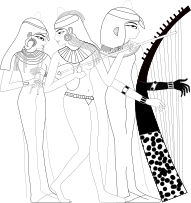
\includegraphics[width=1.5cm]{lettrine-E-trio-degyptiennes.pdf}}\addcontentsline{lof}{figure}{Lettrine \autonym{E} au trio de musiciennes d’après une fresque retrouvée dans la tombe de Nakht à Thèbes.}%
\textsc{coutez !}  La harpe d’Hathor\endnote{Déesse égyptienne de la musique, de l’amour, et de la joie.} est libérée.\endnote{Prononcé par le personnage de la princesse Téti dans le dessin animé qui marqua mon enfance \work{Papyrus} au 16\ieme{} épisode.}\\\nopagebreak[4]
\hspace{0.6cm}Seul le cliquetis de la lance métallique\\\nopagebreak[4]
\hspace{0.6cm}Est instrument lorsqu’il est à terre tombé.
\end{minipage}\\\vspace*{0.4ex}
Tandis que s’étreignent les corps diplomatiques.

Archer, noue ta corde à cette cheville,\\
Avec l’oud rejoins l’orchestre sacré\\
Qui commémore la guerre achevée\\
Quand d’allégresse tressaillent les filles.

Défaisant les sangles corsetant le pied,\\
De ses sandales elle s’est délestée\\
Et dans la marrée elle mouille la jambe\\
D’un mouvement frêle, souple et ingambe.

Monte plus haut réverbe de l’aulos\endnote{Instrument de musique à vent d’Égypte antique.}\\
Dont la Divinité est le présent,\\
Nous éloignant à jamais de l’atroce\\
Par ses parfums exquis et apaisants.

Que les paupières se ferment entrainées par les cils\\
Alourdis des gouttelettes qui abreuvent le Nil\\
De ses généreux torrents d’eau fraîche et intarissable\\
Semblant chaudes lorsqu’elles aspergent nos corps aimables.
\end{verse}


%\chapter{Divers}
%
